%% Time-stamp: <2015-04-30 17:23:24 vk>
%%%% === Disclaimer: =======================================================
%% created by
%%
%%      Karl Voit
%%
%% using GNU/Linux, GNU Emacs & LaTeX 2e
%%

%doc% %% overriding preamble/preamble.tex %%
%doc% \newcommand{\mylinespread}{1.0}  \newcommand{\mycolorlinks}{true}
%doc% \documentclass[12pt,paper=a4,parskip=half,DIV=calc,oneside,%%
%doc% headinclude,footinclude=false,open=right,bibliography=totoc]{scrartcl}
%doc% \usepackage[utf8]{inputenc}\usepackage[ngerman,american]{babel}\usepackage{scrpage2}
%doc% \usepackage{ifthen}\usepackage{eurosym}\usepackage{xspace}\usepackage[usenames,dvipsnames]{xcolor}
%doc% \usepackage[protrusion=true,factor=900]{microtype}
%doc% \usepackage{enumitem}
%doc% \usepackage[pdftex]{graphicx}
%doc% \usepackage{todonotes}
%doc% \usepackage{dingbat,bbding} %% special characters
%doc% \definecolor{DispositionColor}{RGB}{30,103,182}
%doc%
%doc% \usepackage[backend=biber,style=authoryear,dashed=false,natbib=true,hyperref=true%%
%doc% ]{biblatex}
%doc%
%doc% \addbibresource{references-biblatex.bib} %% remove, if using BibTeX instead of biblatex
%doc%
%doc% %% overriding userdata %%
%doc% \newcommand{\myauthor}{Karl Voit}\newcommand{\mytitle}{LaTeX Template Documentation}
%doc% \newcommand{\mysubject}{A Comprehensive Guide to Use the
%doc% Template from https://github.com/novoid/LaTeX-KOMA-template}
%doc% \newcommand{\mykeywords}{LaTeX, pdflatex, template, documentation, biber, biblatex}
%doc%
%doc% \newcommand{\myLaT}{\LaTeX{}@TUG\xspace}
%doc%
%doc% %% for future use?
%doc% % \usepackage{filecontents}
%doc% % \begin{filecontents}{filename.example}
%doc% %
%doc% % \end{filecontents}
%doc%
%doc%
%doc% %% using existing TeX files %%
%doc% %% Time-stamp: <2015-04-30 17:19:58 vk>
%%%% === Disclaimer: =======================================================
%% created by
%%
%%      Karl Voit
%%
%% using GNU/Linux, GNU Emacs & LaTeX 2e
%%

%doc%
%doc% \section{\texttt{mycommands.tex} --- various definitions}\myinteresting
%doc% \label{sec:mycommands}
%doc%
%doc% In file \verb#template/mycommands.tex# many useful commands are being
%doc% defined. 
%doc% 
%doc% \paragraph{What should I do with this file?} Please take a look at its 
%doc% content to get the most out of your document.
%doc% 

%doc% 
%doc% One of the best advantages of \LaTeX{} compared to \myacro{WYSIWYG} software products is
%doc% the possibility to define and use macros within text. This empowers the user to
%doc% a great extend.  Many things can be defined using \verb#\newcommand{}# and
%doc% automates repeating tasks. It is recommended to use macros not only for
%doc% repetitive tasks but also for separating form from content such as \myacro{CSS}
%doc% does for \myacro{XHTML}. Think of including graphics in your document: after
%doc% writing your book, you might want to change all captions to the upper side of
%doc% each figure. In this case you either have to modify all
%doc% \texttt{includegraphics} commands or you were clever enough to define something
%doc% like \verb#\myfig#\footnote{See below for a detailed description}. Using a
%doc% macro for including graphics enables you to modify the position caption on only
%doc% \emph{one} place: at the definition of the macro.
%doc% 
%doc% The following section describes some macros that came with this document template
%doc% from \myLaT and you are welcome to modify or extend them or to create
%doc% your own macros!
%doc% 

%doc% 
%doc% \subsection{\texttt{myfig} --- including graphics made easy}
%doc% 
%doc% The classic: you can easily add graphics to your document with \verb#\myfig#:
%doc% \begin{verbatim}
%doc%  \myfig{flower}%% filename w/o extension in the folder figures
%doc%        {width=0.7\textwidth}%% maximum width/height, aspect ratio will be kept
%doc%        {This flower was photographed at my home town in 2010}%% caption
%doc%        {Home town flower}%% optional (short) caption for list of figures
%doc%        {fig:flower}%% label
%doc% \end{verbatim}
%doc% 
%doc% There are many advantages of this command (compared to manual
%doc% \texttt{figure} environments and \texttt{includegraphics} commands:
%doc% \begin{itemize}
%doc% \item consistent style throughout the whole document
%doc% \item easy to change; for example move caption on top
%doc% \item much less characters to type (faster, error prone)
%doc% \item less visual clutter in the \TeX{}-files
%doc% \end{itemize}
%doc% 
%doc% 
\newcommand{\myfig}[5]{
%% example:
% \myfig{}%% filename in figures folder
%       {width=0.5\textwidth,height=0.5\textheight}%% maximum width/height, aspect ratio will be kept
%       {}%% caption
%       {}%% optional (short) caption for list of figures
%       {}%% label
\begin{figure}%[htp]
  \centering
  \includegraphics[keepaspectratio,#2]{figures/#1}
  \caption[#4]{#3}
  \label{#5} %% NOTE: always label *after* caption!
\end{figure}
}


%doc% 
%doc% \subsection{\texttt{myclone} --- repeat things!}
%doc% 
%doc% Using \verb#\myclone[42]{foobar}# results the text \enquote{foobar} printed 42 times.
%doc% But you can not only repeat text output with \texttt{myclone}. 
%doc%
%doc% Default argument
%doc% for the optional parameter \enquote{number of times} (like \enquote{42} in the example above) 
%doc% is set to two.
%doc% 
%% \myclone[x]{text}
\newcounter{myclonecnt}
\newcommand{\myclone}[2][2]{%
  \setcounter{myclonecnt}{#1}%
  \whiledo{\value{myclonecnt}>0}{#2\addtocounter{myclonecnt}{-1}}%
}

%old% %d oc% 
%old% %d oc% \subsection{\texttt{fixxme} --- sidemark something as unfinished}
%old% %d oc% 
%old% %d oc% You know it: something has to be fixed and you can not do it right
%old% %d oc% now. In order to \texttt{not} forget about it, you might want to add a
%old% %d oc% note like \verb+\fixxme{check again}+ which inserts a note on the page
%old% %d oc% margin such as this\fixxme{check again} example.
%old% %d oc%
%old% \newcommand{\fixxme}[1]{%%
%old% \textcolor{red}{FIXXME}\marginpar{\textcolor{red}{#1}}%%
%old% }


%%%% End 
%%% Local Variables:
%%% mode: latex
%%% mode: auto-fill
%%% mode: flyspell
%%% eval: (ispell-change-dictionary "en_US")
%%% TeX-master: "../main"
%%% End:
%% vim:foldmethod=expr
%% vim:fde=getline(v\:lnum)=~'^%%%%'?0\:getline(v\:lnum)=~'^%doc.*\ .\\%(sub\\)\\?section{.\\+'?'>1'\:'1':

%doc% %%%% Time-stamp: <2015-08-22 17:20:32 vk>
%%%% === Disclaimer: =======================================================
%% created by
%%
%%      Karl Voit
%%
%% using GNU/Linux, GNU Emacs & LaTeX 2e
%%
%doc%
%doc% \section{\texttt{typographic\_settings.tex} --- Typographic finetuning}
%doc%
%doc% The settings of file \verb#template/typographic_settings.tex# contain
%doc% typographic finetuning related to things mentioned in literature.  The
%doc% settings in this file relates to personal taste and most of all: 
%doc% \emph{typographic experience}. 
%doc% 
%doc% \paragraph{What should I do with this file?} You might as well skip the whole
%doc% file by excluding the \verb#%%%% Time-stamp: <2015-08-22 17:20:32 vk>
%%%% === Disclaimer: =======================================================
%% created by
%%
%%      Karl Voit
%%
%% using GNU/Linux, GNU Emacs & LaTeX 2e
%%
%doc%
%doc% \section{\texttt{typographic\_settings.tex} --- Typographic finetuning}
%doc%
%doc% The settings of file \verb#template/typographic_settings.tex# contain
%doc% typographic finetuning related to things mentioned in literature.  The
%doc% settings in this file relates to personal taste and most of all: 
%doc% \emph{typographic experience}. 
%doc% 
%doc% \paragraph{What should I do with this file?} You might as well skip the whole
%doc% file by excluding the \verb#\input{template/typographic_settings.tex}# command
%doc% in \texttt{main.tex}.  For standard usage it is recommended to stay with the
%doc% default settings.
%doc% 
%doc% 
%% ========================================================================

%doc%
%doc% Some basic microtypographic settings are provided by the
%doc% \texttt{microtype}
%doc% package\footnote{\url{http://ctan.org/pkg/microtype}}. This template
%doc% uses the rather conservative package parameters: \texttt{protrusion=true,factor=900}.
\usepackage[protrusion=true,factor=900]{microtype}

%doc%
%doc% \subsection{French spacing}
%doc%
%doc% \paragraph{Why?} see~\textcite[p.\,28, p.\,30]{Bringhurst1993}: `2.1.4 Use a single word space between sentences.'
%doc%
%doc% \paragraph{How?} see~\textcite[p.\,185]{Eijkhout2008}:\\
%doc% \verb#\frenchspacing  %% Macro to switch off extra space after punctuation.# \\
\frenchspacing  %% Macro to switch off extra space after punctuation.
%doc%
%doc% Note: This setting might be default for \myacro{KOMA} script.
%doc%


%doc%
%doc% \subsection{Font}
%doc% 
%doc% This template is using the Palatino font (package \texttt{mathpazo}) which results
%doc% in a legible document and matching mathematical fonts for printout.
%doc% 
%doc% It is highly recommended that you either stick to the Palatino font or use the
%doc% \LaTeX{} default fonts (by removing the package \texttt{mathpazo}).
%doc% 
%doc% Chosing different fonts is not
%doc% an easy task. Please leave this to people with good knowledge on this subject.
%doc% 
%doc% One valid reason to change the default fonts is when your document is mainly
%doc% read on a computer screen. In this case it is recommended to switch to a font
%doc% \textsf{which is sans-serif like this}. This template contains several alternative
%doc% font packages which can be activated in this file.
%doc% 

% for changing the default font, please go to the next subsection!

%doc%
%doc% \subsection{Text figures}
%doc% 
%doc% \ldots also called old style numbers such as 0123456789. 
%doc% (German: \enquote{Mediäval\-ziffern\footnote{\url{https://secure.wikimedia.org/wikibooks/de/wiki/LaTeX-W\%C3\%B6rterbuch:\_Medi\%C3\%A4valziffern}}})
%doc% \paragraph{Why?} see~\textcite[p.\,44f]{Bringhurst1993}: 
%doc% \begin{quote}
%doc% `3.2.1 If the font includes both text figures and titling figures, use
%doc%  titling figures only with full caps, and text figures in all other
%doc%  circumstances.'
%doc% \end{quote}
%doc% 
%doc% \paragraph{How?} 
%doc% Quoted from Wikibooks\footnote{\url{https://secure.wikimedia.org/wikibooks/en/wiki/LaTeX/Formatting\#Text\_figures\_.28.22old\_style.22\_numerals.29}}:
%doc% \begin{quote}
%doc% Some fonts do not have text figures built in; the textcomp package attempts to
%doc% remedy this by effectively generating text figures from the currently-selected
%doc% font. Put \verb#\usepackage{textcomp}# in your preamble. textcomp also allows you to
%doc% use decimal points, properly formatted dollar signs, etc. within
%doc% \verb#\oldstylenums{}#.
%doc% \end{quote}
%doc% \ldots but proposed \LaTeX{} method does not work out well. Instead use:\\
%doc% \verb#\usepackage{hfoldsty}#  (enables text figures using additional font) or \\
%doc% \verb#\usepackage[sc,osf]{mathpazo}# (switches to Palatino font with small caps and old style figures enabled).
%doc%
%\usepackage{hfoldsty}  %% enables text figures using additional font
%% ... OR use ...
\usepackage[sc,osf]{mathpazo} %% switches to Palatino with small caps and old style figures

%% Font selection from:
%%     http://www.matthiaspospiech.de/latex/vorlagen/allgemein/preambel/fonts/
%% use following lines *instead* of the mathpazo package above:
%% ===== Serif =========================================================
%% for Computer Modern (LaTeX default font), simply remove the mathpazo above
%\usepackage{charter}\linespread{1.05} %% Charter
%\usepackage{bookman}                  %% Bookman (laedt Avant Garde !!)
%\usepackage{newcent}                  %% New Century Schoolbook (laedt Avant Garde !!)
%% ===== Sans Serif ====================================================
%\renewcommand{\familydefault}{\sfdefault}  %% this one in *combination* with the default mathpazo package
%\usepackage{cmbright}                  %% CM-Bright (eigntlich eine Familie)
%\usepackage{tpslifonts}                %% tpslifonts % Font for Slides


%doc% 
%doc% \subsection{\texttt{myacro} --- Abbrevations using \textsc{small caps}}\myinteresting
%doc% \label{sec:myacro}
%doc% 
%doc% \paragraph{Why?} see~\textcite[p.\,45f]{Bringhurst1993}: `3.2.2 For abbrevations and
%doc% acronyms in the midst of normal text, use spaced small caps.'
%doc% 
%doc% \paragraph{How?} Using the predefined macro \verb#\myacro{}# for things like
%doc% \myacro{UNO} or \myacro{UNESCO} using \verb#\myacro{UNO}# or \verb#\myacro{UNESCO}#.
%doc% 
\DeclareRobustCommand{\myacro}[1]{\textsc{\lowercase{#1}}} %%  abbrevations using small caps


%doc% 
%doc% \subsection{Colorized headings and links}
%doc% 
%doc% This document template is able to generate an output that uses colorized
%doc% headings, captions, page numbers, and links. The color named `DispositionColor'
%doc% used in this document is defined near the definition of package \texttt{color}
%doc% in the preamble (see section~\ref{subsec:miscpackages}). The changes required
%doc% for headings, page numbers, and captions are defined here.
%doc% 
%doc% Settings for colored links are handled by the definitions of the
%doc% \texttt{hyperref} package (see section~\ref{sec:pdf}).
%doc% 
\setheadsepline{.4pt}[\color{DispositionColor}]
\renewcommand{\headfont}{\normalfont\sffamily\color{DispositionColor}}
\renewcommand{\pnumfont}{\normalfont\sffamily\color{DispositionColor}}
\addtokomafont{disposition}{\color{DispositionColor}}
\addtokomafont{caption}{\color{DispositionColor}\footnotesize}
\addtokomafont{captionlabel}{\color{DispositionColor}}

%doc% 
%doc% \subsection{No figures or tables below footnotes}
%doc% 
%doc% \LaTeX{} places floating environments below footnotes if \texttt{b}
%doc% (bottom) is used as (default) placement algorithm. This is certainly
%doc% not appealing for most people and is deactivated in this template by
%doc% using the package \texttt{footmisc} with its option \texttt{bottom}.
%doc% 
%% see also: http://www.komascript.de/node/858 (German description)
\usepackage[bottom]{footmisc}

%doc% 
%doc% \subsection{Spacings of list environments}
%doc% 
%doc% By default, \LaTeX{} is using vertical spaces between items of enumerate, 
%doc% itemize and description environments. This is fine for multi-line items.
%doc% Many times, the user does just write single-line items where the larger
%doc% vertical space is inappropriate. The \href{http://ctan.org/pkg/enumitem}{enumitem}
%doc% package provides replacements for the pre-defined list environments and
%doc% offers many options to modify their appearances.
%doc% This template is using the package option for \texttt{noitemsep} which
%doc% mimimizes the vertical space between list items.
%doc% 
\usepackage{enumitem}
\setlist{noitemsep}   %% kills the space between items

%doc% 
%doc% \subsection{\texttt{csquotes} --- Correct quotation marks}\myinteresting
%doc% \label{sub:csquotes}
%doc% 
%doc% \emph{Never} use quotation marks found on your keyboard.
%doc% They end up in strange characters or false looking quotation marks.
%doc% 
%doc% In \LaTeX{} you are able to use typographically correct quotation marks. The package 
%doc% \href{http://www.ctan.org/pkg/csquotes}{\texttt{csquotes}} offers you with 
%doc% \verb#\enquote{foobar}# a command to get correct quotation marks around \enquote{foobar}.
%doc% Please do check the package options in order to modify
%doc% its settings according to the language used\footnote{most of the time in 
%doc% combination with the language set in the options of the \texttt{babel} package}.
%doc% 
%doc% \href{http://www.ctan.org/pkg/csquotes}{\texttt{csquotes}} is also recommended 
%doc% by \texttt{biblatex} (see Section~\ref{sec:references}). 
\usepackage[babel=true,strict=true,english=american,german=guillemets]{csquotes}

%doc% 
%doc% \subsection{Line spread}
%doc% 
%doc% If you have to enlarge the distance between two lines of text, you can
%doc% increase it using the \texttt{\mylinespread} command in \texttt{main.tex}. By default, it is
%doc% deactivated (set to 100~percent). Modify only with caution since it influences the
%doc% page layout and could lead to ugly looking documents.
\linespread{\mylinespread}

%doc% 
%doc% \subsection{Optional: Lines above and below the chapter head}
%doc% 
%doc% This is not quite something typographic but rather a matter of taste.
%doc% \myacro{KOMA} Script offers \href{http://www.komascript.de/node/24}{a method to
%doc% add lines above and below chapter head} which is disabled by
%doc% default. If you want to enable this feature, remove corresponding
%doc% comment characters from the settings.
%doc% 
%% Source: http://www.komascript.de/node/24
%disabled% %% 1st get a new command
%disabled% \newcommand*{\ORIGchapterheadstartvskip}{}%
%disabled% %% 2nd save the original definition to the new command
%disabled% \let\ORIGchapterheadstartvskip=\chapterheadstartvskip
%disabled% %% 3rd redefine the command using the saved original command
%disabled% \renewcommand*{\chapterheadstartvskip}{%
%disabled%   \ORIGchapterheadstartvskip
%disabled%   {%
%disabled%     \setlength{\parskip}{0pt}%
%disabled%     \noindent\color{DispositionColor}\rule[.3\baselineskip]{\linewidth}{1pt}\par
%disabled%   }%
%disabled% }
%disabled% %% see above
%disabled% \newcommand*{\ORIGchapterheadendvskip}{}%
%disabled% \let\ORIGchapterheadendvskip=\chapterheadendvskip
%disabled% \renewcommand*{\chapterheadendvskip}{%
%disabled%   {%
%disabled%     \setlength{\parskip}{0pt}%
%disabled%     \noindent\color{DispositionColor}\rule[.3\baselineskip]{\linewidth}{1pt}\par
%disabled%   }%
%disabled%   \ORIGchapterheadendvskip
%disabled% }

%doc% 
%doc% \subsection{Optional: Chapter thumbs}
%doc% 
%doc% This is not quite something typographic but rather a matter of taste.
%doc% \myacro{KOMA} Script offers \href{http://www.komascript.de/chapterthumbs-example}{a method to
%doc% add chapter thumbs} (in combination with the package \texttt{scrpage2}) which is disabled by
%doc% default. If you want to enable this feature, remove corresponding
%doc% comment characters from the settings.
%doc% 
%disabled% \makeatletter
%disabled% % Safty first
%disabled% \@ifundefined{chapter}{\let\chapter\undefined
%disabled%   \chapter must be defined to use chapter thumbs!}{%
%disabled%  
%disabled% % Two new commands for the width and height of the boxes with the
%disabled% % chapter number at the thumbs (use of commands instead of lengths
%disabled% % for sparing registers)
%disabled% \newcommand*{\chapterthumbwidth}{2em}
%disabled% \newcommand*{\chapterthumbheight}{1em}
%disabled%  
%disabled% % Two new commands for the colors of the box background and the
%disabled% % chapter numbers of the thumbs
%disabled% \newcommand*{\chapterthumbboxcolor}{black}
%disabled% \newcommand*{\chapterthumbtextcolor}{white}
%disabled%  
%disabled% % New command to set a chapter thumb. I'm using a group at this
%disabled% % command, because I'm changing the temporary dimension \@tempdima
%disabled% \newcommand*{\putchapterthumb}{%
%disabled%   \begingroup
%disabled%     \Large
%disabled%     % calculate the horizontal possition of the right paper border
%disabled%     % (I ignore \hoffset, because I interprete \hoffset moves the page
%disabled%     % at the paper e.g. if you are using cropmarks)
%disabled%     \setlength{\@tempdima}{\@oddheadshift}% (internal from scrpage2)
%disabled%     \setlength{\@tempdima}{-\@tempdima}%
%disabled%     \addtolength{\@tempdima}{\paperwidth}%
%disabled%     \addtolength{\@tempdima}{-\oddsidemargin}%
%disabled%     \addtolength{\@tempdima}{-1in}%
%disabled%     % putting the thumbs should not change the horizontal
%disabled%     % possition
%disabled%     \rlap{%
%disabled%       % move to the calculated horizontal possition
%disabled%       \hspace*{\@tempdima}%
%disabled%       % putting the thumbs should not change the vertical
%disabled%       % possition
%disabled%       \vbox to 0pt{%
%disabled%         % calculate the vertical possition of the thumbs (I ignore
%disabled%         % \voffset for the same reasons told above)
%disabled%         \setlength{\@tempdima}{\chapterthumbwidth}%
%disabled%         \multiply\@tempdima by\value{chapter}%
%disabled%         \addtolength{\@tempdima}{-\chapterthumbwidth}%
%disabled%         \addtolength{\@tempdima}{-\baselineskip}%
%disabled%         % move to the calculated vertical possition
%disabled%         \vspace*{\@tempdima}%
%disabled%         % put the thumbs left so the current horizontal possition
%disabled%         \llap{%
%disabled%           % and rotate them
%disabled%           \rotatebox{90}{\colorbox{\chapterthumbboxcolor}{%
%disabled%               \parbox[c][\chapterthumbheight][c]{\chapterthumbwidth}{%
%disabled%                 \centering
%disabled%                 \textcolor{\chapterthumbtextcolor}{%
%disabled%                   \strut\thechapter}\\
%disabled%               }%
%disabled%             }%
%disabled%           }%
%disabled%         }%
%disabled%         % avoid overfull \vbox messages
%disabled%         \vss
%disabled%       }%
%disabled%     }%
%disabled%   \endgroup
%disabled% }
%disabled%  
%disabled% % New command, which works like \lohead but also puts the thumbs (you
%disabled% % cannot use \ihead with this definition but you may change this, if
%disabled% % you use more internal scrpage2 commands)
%disabled% \newcommand*{\loheadwithchapterthumbs}[2][]{%
%disabled%   \lohead[\putchapterthumb#1]{\putchapterthumb#2}%
%disabled% }
%disabled%  
%disabled% % initial use
%disabled% \loheadwithchapterthumbs{}
%disabled% \pagestyle{scrheadings}
%disabled%  
%disabled% }
%disabled% \makeatother

%%%% END
%%% Local Variables:
%%% mode: latex
%%% mode: auto-fill
%%% mode: flyspell
%%% eval: (ispell-change-dictionary "en_US")
%%% TeX-master: "../main"
%%% End:
%% vim:foldmethod=expr
%% vim:fde=getline(v\:lnum)=~'^%%%%'?0\:getline(v\:lnum)=~'^%doc.*\ .\\%(sub\\)\\?section{.\\+'?'>1'\:'1':
# command
%doc% in \texttt{main.tex}.  For standard usage it is recommended to stay with the
%doc% default settings.
%doc% 
%doc% 
%% ========================================================================

%doc%
%doc% Some basic microtypographic settings are provided by the
%doc% \texttt{microtype}
%doc% package\footnote{\url{http://ctan.org/pkg/microtype}}. This template
%doc% uses the rather conservative package parameters: \texttt{protrusion=true,factor=900}.
\usepackage[protrusion=true,factor=900]{microtype}

%doc%
%doc% \subsection{French spacing}
%doc%
%doc% \paragraph{Why?} see~\textcite[p.\,28, p.\,30]{Bringhurst1993}: `2.1.4 Use a single word space between sentences.'
%doc%
%doc% \paragraph{How?} see~\textcite[p.\,185]{Eijkhout2008}:\\
%doc% \verb#\frenchspacing  %% Macro to switch off extra space after punctuation.# \\
\frenchspacing  %% Macro to switch off extra space after punctuation.
%doc%
%doc% Note: This setting might be default for \myacro{KOMA} script.
%doc%


%doc%
%doc% \subsection{Font}
%doc% 
%doc% This template is using the Palatino font (package \texttt{mathpazo}) which results
%doc% in a legible document and matching mathematical fonts for printout.
%doc% 
%doc% It is highly recommended that you either stick to the Palatino font or use the
%doc% \LaTeX{} default fonts (by removing the package \texttt{mathpazo}).
%doc% 
%doc% Chosing different fonts is not
%doc% an easy task. Please leave this to people with good knowledge on this subject.
%doc% 
%doc% One valid reason to change the default fonts is when your document is mainly
%doc% read on a computer screen. In this case it is recommended to switch to a font
%doc% \textsf{which is sans-serif like this}. This template contains several alternative
%doc% font packages which can be activated in this file.
%doc% 

% for changing the default font, please go to the next subsection!

%doc%
%doc% \subsection{Text figures}
%doc% 
%doc% \ldots also called old style numbers such as 0123456789. 
%doc% (German: \enquote{Mediäval\-ziffern\footnote{\url{https://secure.wikimedia.org/wikibooks/de/wiki/LaTeX-W\%C3\%B6rterbuch:\_Medi\%C3\%A4valziffern}}})
%doc% \paragraph{Why?} see~\textcite[p.\,44f]{Bringhurst1993}: 
%doc% \begin{quote}
%doc% `3.2.1 If the font includes both text figures and titling figures, use
%doc%  titling figures only with full caps, and text figures in all other
%doc%  circumstances.'
%doc% \end{quote}
%doc% 
%doc% \paragraph{How?} 
%doc% Quoted from Wikibooks\footnote{\url{https://secure.wikimedia.org/wikibooks/en/wiki/LaTeX/Formatting\#Text\_figures\_.28.22old\_style.22\_numerals.29}}:
%doc% \begin{quote}
%doc% Some fonts do not have text figures built in; the textcomp package attempts to
%doc% remedy this by effectively generating text figures from the currently-selected
%doc% font. Put \verb#\usepackage{textcomp}# in your preamble. textcomp also allows you to
%doc% use decimal points, properly formatted dollar signs, etc. within
%doc% \verb#\oldstylenums{}#.
%doc% \end{quote}
%doc% \ldots but proposed \LaTeX{} method does not work out well. Instead use:\\
%doc% \verb#\usepackage{hfoldsty}#  (enables text figures using additional font) or \\
%doc% \verb#\usepackage[sc,osf]{mathpazo}# (switches to Palatino font with small caps and old style figures enabled).
%doc%
%\usepackage{hfoldsty}  %% enables text figures using additional font
%% ... OR use ...
\usepackage[sc,osf]{mathpazo} %% switches to Palatino with small caps and old style figures

%% Font selection from:
%%     http://www.matthiaspospiech.de/latex/vorlagen/allgemein/preambel/fonts/
%% use following lines *instead* of the mathpazo package above:
%% ===== Serif =========================================================
%% for Computer Modern (LaTeX default font), simply remove the mathpazo above
%\usepackage{charter}\linespread{1.05} %% Charter
%\usepackage{bookman}                  %% Bookman (laedt Avant Garde !!)
%\usepackage{newcent}                  %% New Century Schoolbook (laedt Avant Garde !!)
%% ===== Sans Serif ====================================================
%\renewcommand{\familydefault}{\sfdefault}  %% this one in *combination* with the default mathpazo package
%\usepackage{cmbright}                  %% CM-Bright (eigntlich eine Familie)
%\usepackage{tpslifonts}                %% tpslifonts % Font for Slides


%doc% 
%doc% \subsection{\texttt{myacro} --- Abbrevations using \textsc{small caps}}\myinteresting
%doc% \label{sec:myacro}
%doc% 
%doc% \paragraph{Why?} see~\textcite[p.\,45f]{Bringhurst1993}: `3.2.2 For abbrevations and
%doc% acronyms in the midst of normal text, use spaced small caps.'
%doc% 
%doc% \paragraph{How?} Using the predefined macro \verb#\myacro{}# for things like
%doc% \myacro{UNO} or \myacro{UNESCO} using \verb#\myacro{UNO}# or \verb#\myacro{UNESCO}#.
%doc% 
\DeclareRobustCommand{\myacro}[1]{\textsc{\lowercase{#1}}} %%  abbrevations using small caps


%doc% 
%doc% \subsection{Colorized headings and links}
%doc% 
%doc% This document template is able to generate an output that uses colorized
%doc% headings, captions, page numbers, and links. The color named `DispositionColor'
%doc% used in this document is defined near the definition of package \texttt{color}
%doc% in the preamble (see section~\ref{subsec:miscpackages}). The changes required
%doc% for headings, page numbers, and captions are defined here.
%doc% 
%doc% Settings for colored links are handled by the definitions of the
%doc% \texttt{hyperref} package (see section~\ref{sec:pdf}).
%doc% 
\setheadsepline{.4pt}[\color{DispositionColor}]
\renewcommand{\headfont}{\normalfont\sffamily\color{DispositionColor}}
\renewcommand{\pnumfont}{\normalfont\sffamily\color{DispositionColor}}
\addtokomafont{disposition}{\color{DispositionColor}}
\addtokomafont{caption}{\color{DispositionColor}\footnotesize}
\addtokomafont{captionlabel}{\color{DispositionColor}}

%doc% 
%doc% \subsection{No figures or tables below footnotes}
%doc% 
%doc% \LaTeX{} places floating environments below footnotes if \texttt{b}
%doc% (bottom) is used as (default) placement algorithm. This is certainly
%doc% not appealing for most people and is deactivated in this template by
%doc% using the package \texttt{footmisc} with its option \texttt{bottom}.
%doc% 
%% see also: http://www.komascript.de/node/858 (German description)
\usepackage[bottom]{footmisc}

%doc% 
%doc% \subsection{Spacings of list environments}
%doc% 
%doc% By default, \LaTeX{} is using vertical spaces between items of enumerate, 
%doc% itemize and description environments. This is fine for multi-line items.
%doc% Many times, the user does just write single-line items where the larger
%doc% vertical space is inappropriate. The \href{http://ctan.org/pkg/enumitem}{enumitem}
%doc% package provides replacements for the pre-defined list environments and
%doc% offers many options to modify their appearances.
%doc% This template is using the package option for \texttt{noitemsep} which
%doc% mimimizes the vertical space between list items.
%doc% 
\usepackage{enumitem}
\setlist{noitemsep}   %% kills the space between items

%doc% 
%doc% \subsection{\texttt{csquotes} --- Correct quotation marks}\myinteresting
%doc% \label{sub:csquotes}
%doc% 
%doc% \emph{Never} use quotation marks found on your keyboard.
%doc% They end up in strange characters or false looking quotation marks.
%doc% 
%doc% In \LaTeX{} you are able to use typographically correct quotation marks. The package 
%doc% \href{http://www.ctan.org/pkg/csquotes}{\texttt{csquotes}} offers you with 
%doc% \verb#\enquote{foobar}# a command to get correct quotation marks around \enquote{foobar}.
%doc% Please do check the package options in order to modify
%doc% its settings according to the language used\footnote{most of the time in 
%doc% combination with the language set in the options of the \texttt{babel} package}.
%doc% 
%doc% \href{http://www.ctan.org/pkg/csquotes}{\texttt{csquotes}} is also recommended 
%doc% by \texttt{biblatex} (see Section~\ref{sec:references}). 
\usepackage[babel=true,strict=true,english=american,german=guillemets]{csquotes}

%doc% 
%doc% \subsection{Line spread}
%doc% 
%doc% If you have to enlarge the distance between two lines of text, you can
%doc% increase it using the \texttt{\mylinespread} command in \texttt{main.tex}. By default, it is
%doc% deactivated (set to 100~percent). Modify only with caution since it influences the
%doc% page layout and could lead to ugly looking documents.
\linespread{\mylinespread}

%doc% 
%doc% \subsection{Optional: Lines above and below the chapter head}
%doc% 
%doc% This is not quite something typographic but rather a matter of taste.
%doc% \myacro{KOMA} Script offers \href{http://www.komascript.de/node/24}{a method to
%doc% add lines above and below chapter head} which is disabled by
%doc% default. If you want to enable this feature, remove corresponding
%doc% comment characters from the settings.
%doc% 
%% Source: http://www.komascript.de/node/24
%disabled% %% 1st get a new command
%disabled% \newcommand*{\ORIGchapterheadstartvskip}{}%
%disabled% %% 2nd save the original definition to the new command
%disabled% \let\ORIGchapterheadstartvskip=\chapterheadstartvskip
%disabled% %% 3rd redefine the command using the saved original command
%disabled% \renewcommand*{\chapterheadstartvskip}{%
%disabled%   \ORIGchapterheadstartvskip
%disabled%   {%
%disabled%     \setlength{\parskip}{0pt}%
%disabled%     \noindent\color{DispositionColor}\rule[.3\baselineskip]{\linewidth}{1pt}\par
%disabled%   }%
%disabled% }
%disabled% %% see above
%disabled% \newcommand*{\ORIGchapterheadendvskip}{}%
%disabled% \let\ORIGchapterheadendvskip=\chapterheadendvskip
%disabled% \renewcommand*{\chapterheadendvskip}{%
%disabled%   {%
%disabled%     \setlength{\parskip}{0pt}%
%disabled%     \noindent\color{DispositionColor}\rule[.3\baselineskip]{\linewidth}{1pt}\par
%disabled%   }%
%disabled%   \ORIGchapterheadendvskip
%disabled% }

%doc% 
%doc% \subsection{Optional: Chapter thumbs}
%doc% 
%doc% This is not quite something typographic but rather a matter of taste.
%doc% \myacro{KOMA} Script offers \href{http://www.komascript.de/chapterthumbs-example}{a method to
%doc% add chapter thumbs} (in combination with the package \texttt{scrpage2}) which is disabled by
%doc% default. If you want to enable this feature, remove corresponding
%doc% comment characters from the settings.
%doc% 
%disabled% \makeatletter
%disabled% % Safty first
%disabled% \@ifundefined{chapter}{\let\chapter\undefined
%disabled%   \chapter must be defined to use chapter thumbs!}{%
%disabled%  
%disabled% % Two new commands for the width and height of the boxes with the
%disabled% % chapter number at the thumbs (use of commands instead of lengths
%disabled% % for sparing registers)
%disabled% \newcommand*{\chapterthumbwidth}{2em}
%disabled% \newcommand*{\chapterthumbheight}{1em}
%disabled%  
%disabled% % Two new commands for the colors of the box background and the
%disabled% % chapter numbers of the thumbs
%disabled% \newcommand*{\chapterthumbboxcolor}{black}
%disabled% \newcommand*{\chapterthumbtextcolor}{white}
%disabled%  
%disabled% % New command to set a chapter thumb. I'm using a group at this
%disabled% % command, because I'm changing the temporary dimension \@tempdima
%disabled% \newcommand*{\putchapterthumb}{%
%disabled%   \begingroup
%disabled%     \Large
%disabled%     % calculate the horizontal possition of the right paper border
%disabled%     % (I ignore \hoffset, because I interprete \hoffset moves the page
%disabled%     % at the paper e.g. if you are using cropmarks)
%disabled%     \setlength{\@tempdima}{\@oddheadshift}% (internal from scrpage2)
%disabled%     \setlength{\@tempdima}{-\@tempdima}%
%disabled%     \addtolength{\@tempdima}{\paperwidth}%
%disabled%     \addtolength{\@tempdima}{-\oddsidemargin}%
%disabled%     \addtolength{\@tempdima}{-1in}%
%disabled%     % putting the thumbs should not change the horizontal
%disabled%     % possition
%disabled%     \rlap{%
%disabled%       % move to the calculated horizontal possition
%disabled%       \hspace*{\@tempdima}%
%disabled%       % putting the thumbs should not change the vertical
%disabled%       % possition
%disabled%       \vbox to 0pt{%
%disabled%         % calculate the vertical possition of the thumbs (I ignore
%disabled%         % \voffset for the same reasons told above)
%disabled%         \setlength{\@tempdima}{\chapterthumbwidth}%
%disabled%         \multiply\@tempdima by\value{chapter}%
%disabled%         \addtolength{\@tempdima}{-\chapterthumbwidth}%
%disabled%         \addtolength{\@tempdima}{-\baselineskip}%
%disabled%         % move to the calculated vertical possition
%disabled%         \vspace*{\@tempdima}%
%disabled%         % put the thumbs left so the current horizontal possition
%disabled%         \llap{%
%disabled%           % and rotate them
%disabled%           \rotatebox{90}{\colorbox{\chapterthumbboxcolor}{%
%disabled%               \parbox[c][\chapterthumbheight][c]{\chapterthumbwidth}{%
%disabled%                 \centering
%disabled%                 \textcolor{\chapterthumbtextcolor}{%
%disabled%                   \strut\thechapter}\\
%disabled%               }%
%disabled%             }%
%disabled%           }%
%disabled%         }%
%disabled%         % avoid overfull \vbox messages
%disabled%         \vss
%disabled%       }%
%disabled%     }%
%disabled%   \endgroup
%disabled% }
%disabled%  
%disabled% % New command, which works like \lohead but also puts the thumbs (you
%disabled% % cannot use \ihead with this definition but you may change this, if
%disabled% % you use more internal scrpage2 commands)
%disabled% \newcommand*{\loheadwithchapterthumbs}[2][]{%
%disabled%   \lohead[\putchapterthumb#1]{\putchapterthumb#2}%
%disabled% }
%disabled%  
%disabled% % initial use
%disabled% \loheadwithchapterthumbs{}
%disabled% \pagestyle{scrheadings}
%disabled%  
%disabled% }
%disabled% \makeatother

%%%% END
%%% Local Variables:
%%% mode: latex
%%% mode: auto-fill
%%% mode: flyspell
%%% eval: (ispell-change-dictionary "en_US")
%%% TeX-master: "../main"
%%% End:
%% vim:foldmethod=expr
%% vim:fde=getline(v\:lnum)=~'^%%%%'?0\:getline(v\:lnum)=~'^%doc.*\ .\\%(sub\\)\\?section{.\\+'?'>1'\:'1':

%doc% %%%% Time-stamp: <2014-03-23 13:40:59 vk>
%%%% === Disclaimer: =======================================================
%% created by
%%
%%      Karl Voit
%%
%% using GNU/Linux, GNU Emacs & LaTeX 2e
%%

%doc%
%doc% \section{\texttt{pdf\_settings.tex} --- Settings related to PDF output}
%doc% \label{sec:pdf}
%doc% 
%doc% The file \verb#template/pdf_settings.tex# basically contains the definitions for
%doc% the \href{http://tug.org/applications/hyperref/}{\texttt{hyperref} package}
%doc% including the
%doc% \href{http://www.ctan.org/tex-archive/macros/latex/required/graphics/}{\texttt{graphicx}
%doc% package}. Since these settings should be the last things of any \LaTeX{}
%doc% preamble, they got their own \TeX{} file which is included in \texttt{main.tex}.
%doc% 
%doc% \paragraph{What should I do with this file?} The settings in this file are
%doc% important for \myacro{PDF} output and including graphics. Do not exclude the
%doc% related \texttt{input} command in \texttt{main.tex}. But you might want to
%doc% modify some settings after you read the
%doc% \href{http://tug.org/applications/hyperref/}{documentation of the \texttt{hyperref} package}.
%doc% 


%% Fix positioning of images in PDF viewers. (disabled by
%% default; see https://github.com/novoid/LaTeX-KOMA-template/issues/4
%% for more information) 
%% I do not have time to read about possible side-effect of this
%% package for now.
% \usepackage[hypcap]{caption}

%% Declarations of hyperref should be the last definitions of the preamble:
%% FIXXME: black-and-white-version for printing!

\pdfcompresslevel=9

\usepackage[%
unicode=true, % loads with unicode support
%a4paper=true, %
pdftex=true, %
backref, %
pagebackref=false, % creates backward references too
bookmarks=false, %
bookmarksopen=false, % when starting with AcrobatReader, the Bookmarkcolumn is opened
pdfpagemode=None,% None, UseOutlines, UseThumbs, FullScreen
plainpages=false, % correct, if pdflatex complains: ``destination with same identifier already exists''
%% colors: https://secure.wikimedia.org/wikibooks/en/wiki/LaTeX/Colors
urlcolor=DispositionColor, %%
linkcolor=DispositionColor, %%
pagecolor=DispositionColor, %%
citecolor=DispositionColor, %%
anchorcolor=DispositionColor, %%
colorlinks=\mycolorlinks, % turn on/off colored links (on: better for
                          % on-screen reading; off: better for printout versions)
]{hyperref}

%% all strings need to be loaded after hyperref was loaded with unicode support
%% if not the field is garbled in the output for characters like ČŽĆŠĐ
\hypersetup{
pdftitle={\mytitle}, %
pdfauthor={\myauthor}, %
pdfsubject={\mysubject}, %
pdfcreator={Accomplished with: pdfLaTeX, biber, and hyperref-package. No animals, MS-EULA or BSA-rules were harmed.},
pdfproducer={\myauthor},
pdfkeywords={\mykeywords}
}

%\DeclareGraphicsExtensions{.pdf}

%%%% END
%%% Local Variables:
%%% TeX-master: "../main"
%%% mode: latex
%%% mode: auto-fill
%%% mode: flyspell
%%% eval: (ispell-change-dictionary "en_US")
%%% End:
%% vim:foldmethod=expr
%% vim:fde=getline(v\:lnum)=~'^%%%%'?0\:getline(v\:lnum)=~'^%doc.*\ .\\%(sub\\)\\?section{.\\+'?'>1'\:'1':

%doc%
%doc% \begin{document}
%doc% %% title page %%
%doc% \title{\mytitle}\subtitle{\mysubject}
%doc% \author{\myauthor}
%doc% \date{\today}
%doc%
%doc% \maketitle\newpage
%doc%
%doc% \tableofcontents\newpage
%doc% %%---------------------------------------%%

%doc%
%doc% \section{How to use this \LaTeX{} document template}
%doc%
%doc% This \LaTeX{} document template from
%doc% \myLaT\footnote{\url{http://LaTeX.TUGraz.at}} is based on \myacro{KOMA}
%doc% script\footnote{\url{http://komascript.de/}}. You don't need any
%doc% special \myacro{KOMA} knowledge (but it woun't hurt either). It provides an easy to use and
%doc% easy to modify template. All settings are documented and many references to
%doc% additional information sources are given.
%doc%

%doc% In general, there should not be any reason to modify a file in
%doc% the \texttt{template} folder. \emph{All important settings are
%doc% accessible in the main folder, mostly in the \texttt{main.tex}
%doc% file.} This way, it is easy to get what you need and you can update
%doc% the template independent of the content of the document.
%doc%
%doc% \newcommand{\myimportant}{%% mark important chapters
%doc%   \marginpar{\vspace{-1em}\rightpointleft}
%doc% }
%doc% \newcommand{\myinteresting}{\marginpar{\vspace{-2em}\PencilLeftDown}}

%doc%
%doc% The \emph{absolute minimum you should read} is listed below and
%doc% marked with the hand symbol:\myimportant
%doc% \begin{itemize}
%doc% \item Section~\ref{sec:modifytemplate}: basic configuration of this template.
%doc% \item Section~\ref{sec:howtocompile}: how to generate the \myacro{PDF} file
%doc% \item Section~\ref{sec:references}: using biblatex (instead of bibtex)
%doc% \end{itemize}
%doc%
%doc% In order to get a perfect resulting document and to get an
%doc% exciting experience with this template, you should definitely consider reading
%doc% following sections which are also marked with the pencil symbol:\myinteresting
%doc% \begin{itemize}
%doc% \item Section~\ref{sec:extending-template}: extend the template with
%doc%   your own usepackages, newcommands, and so forth
%doc% \item Section~\ref{sec:mycommands}: pre-defined commands to make your life easier (e.g., including graphics)
%doc% \item Section~\ref{sec:myacro}: how to do acronyms (like \myacro{ACME}) beautifully
%doc% \item Section~\ref{sub:csquotes}: how to \enquote{quote} text and use parentheses correctly
%doc% \end{itemize}
%doc%
%doc% The other sections describe all other settings for the sake of completeness. This is
%doc% interesting for learning more about \LaTeX{} and modifying this template to a higher level of detail.

%doc%
%doc% \newpage
%doc% \subsection{Six Steps to Customize Your Document}\myimportant
%doc% \label{sec:modifytemplate}
%doc%
%doc% This template is optimized to get to the first draft of your thesis
%doc% very quickly. Follow these instructions and you get most of your
%doc% customizing done in a few minutes:
%doc%
%doc% \newcommand{\myfile}[1]{\texttt{\href{file:#1}{#1}}}
%doc%
%doc% \begin{enumerate}
%doc% \item Modify settings in \texttt{main.tex} to meet your requirements:
%doc%   \begin{itemize}
%doc%   \item Basic settings
%doc%     \begin{itemize}
%doc%     \item Paper size, languages, font size, citation style,
%doc%           title page, and so forth
%doc%     \end{itemize}
%doc%   \item Document metadata
%doc%     \begin{itemize}
%doc%     \item Preferences like \verb+myauthor+, \verb+mytitle+, and so forth
%doc%     \end{itemize}
%doc%   \end{itemize}
%doc% \item Replace \myfile{figures/institution.pdf} with the logo of
%doc% your institution in either \myacro{PDF} or \myacro{PNG}
%doc% format.\footnote{Avoid \myacro{JPEG} format for
%doc% computer-generated (pixcel-oriented) graphics like logos or
%doc% screenshots in general. The \myacro{JEPG} format is for
%doc% photographs \emph{only}.}
%doc% \item Further down in \myfile{main.tex}:
%doc%   \begin{itemize}
%doc%   \item Create your desired structure for the chapters
%doc%         (\verb+\chapter{Introduction}

TODO Ask the question that will be solved by this thesis
e.g. "What is the impact of using best practice software architecture patterns over ad-hoc monilithic software development?"+, \verb+\include{evaluation}+, \ldots)
%doc%   \end{itemize}
%doc% \item Create the \TeX{} files and fill your content into these files you defined in the previous step.
%doc% \item Optionally: Modify \myfile{colophon.tex} to meet your situation.
%doc%   \begin{itemize}
%doc%   \item Please spend a couple of minutes and think about putting your work
%doc%         under an open license\footnote{\url{https://creativecommons.org/licenses/}}
%doc%         in order to follow the spirit of Open Science\footnote{\url{https://en.wikipedia.org/wiki/Open_science}}.
%doc%   \end{itemize}
%doc% \item In case you are using \myacro{GNU} make\footnote{If you
%doc%       don't know, what \myacro{GNU} make is, you are not using it (yet).}:
%doc%       Put your desired \myacro{PDF} file name in the second line of file
%doc%    \myfile{Makefile}
%doc%    \begin{itemize}
%doc%    \item replace \enquote{Projectname} with your filename
%doc%    \item do not use any file extension like \texttt{.tex} or \texttt{.pdf}
%doc%    \end{itemize}
%doc% \end{enumerate}
%doc%
%doc%

%doc%
%doc% \subsection{License}\myimportant
%doc% \label{sec:license}
%doc%
%doc% This template is licensed under a Creative Commons Attribution-ShareAlike 3.0 Unported (CC BY-SA 3.0)
%doc%         license\footnote{\url{https://creativecommons.org/licenses/by-sa/3.0/}}:
%doc%     \begin{itemize}
%doc%     \item You can share (to copy, distribute and transmit) this template.
%doc%     \item You can remix (adapt) this template.
%doc%     \item You can make commercial use of the template.
%doc%     \item In case you modify this template and share the derived
%doc%           template: You must attribute the template such that you do not
%doc%           remove (co-)authorship of Karl Voit and you must not remove
%doc%           the URL to the original repository on
%doc%           github\footnote{\url{https://github.com/novoid/LaTeX-KOMA-template}}.
%doc%     \item If you alter, transform, or build a new template upon
%doc%           this template, you may distribute the resulting
%doc%           template only under the same or similar license to this one.
%doc%     \item There are \emph{no restrictions} of any kind, however, related to the
%doc%           resulting (PDF) document!
%doc%     \item You may remove the colophon (but it's not recommended).
%doc%     \end{itemize}


%doc%
%doc%
%doc% \subsection{How to compile this document}\myimportant
%doc% \label{sec:howtocompile}
%doc%
%doc% I assume that compiling \LaTeX{} documents within your software
%doc% environment is something you have already learned. This template is
%doc% almost like any other \LaTeX{} document except it uses
%doc% state-of-the-art tools for generating things like the list of
%doc% references using biblatex/biber (see
%doc% Section~\ref{sec:references} for details). Unfortunately, some \LaTeX{} editors
%doc% do not support this much better way of working with bibliography
%doc% references yet. This section describes how to compile this template.
%doc%
%doc% \subsubsection{Compiling Using a \LaTeX{} Editor}
%doc%
%doc% Please do select \myfile{main.tex} as the \enquote{main project file} or make
%doc% sure to compile/run only \myfile{main.tex} (and not \myfile{introduction.tex}
%doc% or other \TeX{} files of this template).
%doc%
%doc% Choose \texttt{biber} for generating the references. Modern LaTeX{}
%doc% environments offer this option. Older tools might not be that up to
%doc% date yet.
%doc%

%doc% \subsubsection{Activating \texttt{biber} in the \LaTeX{} editor TeXworks}
%doc% \label{sec:biberTeXworks}
%doc%
%doc% The \href{https://www.tug.org/texworks/}{TeXworks} editor is a very
%doc% basic (but fine) \LaTeX{} editor to start with. It is included in
%doc% \href{http://miktex.org/}{MiKTeX} and
%doc% \href{http://miktex.org/portable}{MiKTeX portable} and supports
%doc% \href{https://en.wikipedia.org/wiki/Syntax_highlighting}{syntax
%doc%   highlighting} and
%doc% \href{http://itexmac.sourceforge.net/SyncTeX.html}{SyncTeX} to
%doc% synchronize \myacro{PDF} output and \LaTeX{} source code.
%doc%
%doc% Unfortunately, TeXworks shipped with MiKTeX does not support compiling
%doc% using \texttt{biber} (biblatex) out of the box. Here is a solution to
%doc% this issue. Go to TeXworks: \texttt{Edit} $\rightarrow$
%doc% \texttt{Preferences~\ldots} $\rightarrow$ \texttt{Typesetting} $\rightarrow$
%doc% \texttt{Processing tools} and add a new entry (using the plus icon):
%doc%
%doc% \begin{tabbing}
%doc%   Arguments: \= foobar  \kill
%doc%   Name:      \> \verb#pdflatex+biber# \\
%doc%   Program:   \> \emph{find the \texttt{template/pdflatex+biber.bat} file from your disk} \\
%doc%   Arguments: \> \verb+$fullname+ \\
%doc%              \> \verb+$basename+
%doc% \end{tabbing}
%doc%
%doc% Activate the \enquote{View PDF after running} option.
%doc%
%doc% Close the preferences dialog and you will now have an additional
%doc% choice in the drop down list for compiling your document. Choose the
%doc% new entry called \verb#pdflatex+biber# and start a happier life with
%doc% \texttt{biber}.
%doc%
%doc% In case your TeXworks has a German user interface, here the key
%doc% aspects in German as well:
%doc%
%doc% \begin{otherlanguage}{ngerman}
%doc%
%doc%   \texttt{Bearbeiten} $\rightarrow$ \texttt{Einstellungen~\ldots} $\rightarrow$
%doc%   \texttt{Textsatz} $\rightarrow$ \texttt{Verarbeitungsprogramme} $\rightarrow$
%doc%   + \emph{(neues Verarbeitungsprogramm)}:
%doc%
%doc% \begin{tabbing}
%doc%   Befehl/Datei: \= foobar  \kill
%doc%     Name: \> pdflatex+biber \\
%doc%     Befehl/Datei: \> \emph{die \texttt{template/pdflatex+biber.bat} im Laufwerk suchen} \\
%doc%     Argumente: \> \verb+$fullname+ \\
%doc%                \> \verb+$basename+
%doc% \end{tabbing}
%doc%
%doc% \enquote{PDF nach Beendigung anzeigen} aktivieren.
%doc%
%doc% \end{otherlanguage}
%doc%

%doc% \subsubsection{Compiling Using \myacro{GNU} make}
%doc%
%doc% With \myacro{GNU}
%doc% make\footnote{\url{https://secure.wikimedia.org/wikipedia/en/wiki/Make\_\%28software\%29}}
%doc% it is just simple as that: \texttt{make pdf}
%doc%
%doc% Several other targets are available. You can check them out by
%doc% executing: \texttt{make help}
%doc%
%doc% In case you are using TeXLive (instead of MiKTeX as I do), you might
%doc% want to modify the line \texttt{PDFLATEX\_CMD = pdflatex} within
%doc% the file \texttt{Makefile} to: \texttt{PDFLATEX\_CMD = pdflatex -synctex=1 -undump=pdflatex}
%doc%
%doc%

%doc% \subsubsection{Compiling in a Text-Shell}
%doc%
%doc% To generate a document using \texttt{Biber}, you can stick to
%doc% following example:
%doc% \begin{verbatim}
%doc% pdflatex main.tex
%doc% biber main
%doc% pdflatex main.tex
%doc% pdflatex main.tex
%doc% \end{verbatim}
%doc% 
%doc% Users of TeXLive with Microsoft Windows might want to try the
%doc% following script\footnote{Thanks to Florian Brucker for provinding
%doc%   this script.} which could be stored as, e.g., \texttt{compile.bat}:
%doc% \begin{verbatim}
%doc% REM call pdflatex using parameters suitable for TeXLive:
%doc% pdflatex.exe  "main.tex"
%doc% REM generate the references metadata for biblatex (using biber):
%doc% biber.exe "main"
%doc% REM call pdflatex twice to compile the references and finalize PDF:
%doc% pdflatex.exe  "main.tex"
%doc% pdflatex.exe -synctex=-1 -interaction=nonstopmode "main.tex"
%doc% \end{verbatim}
%doc% 


%doc%
%doc% \subsection{How to get rid of the template documentation}
%doc%
%doc% Simply remove the files \verb#Template_Documentation.pdf# and
%doc% \verb#Template_Documentation.tex# (if it exists) in the main folder
%doc% of this template.
%doc%
%doc% \subsection{What about modifying or extending the template?}\myinteresting
%doc% \label{sec:extending-template}
%doc%
%doc% This template provides an easy to start \LaTeX{} document template with sound
%doc% default settings. You can modify each setting any time. It is recommended that
%doc% you are familiar with the documentation of the command whose settings you want
%doc% to modify.
%doc%
%doc% It is recommended that for \emph{adding} things to the preambel (newcommands,
%doc% setting variables, defining headers, \dots) you should use the file
%doc% \texttt{main.tex}.
%doc% There are comment lines which help you find the right spot.
%doc% This way you still have the chance to update your \texttt{template}
%doc% folder from the template repository without losing your own added things.
%doc%
%doc% The following sections describe the settings and commands of this template and
%doc% give a short overview of its features.

%doc% \subsection{How to change the title page}
%doc%
%doc% This template comes with a variety of title pages. They are located in
%doc% the folder \texttt{template}. You can switch to a specific title
%doc% page by including the corresponding title page file in the file
%doc% \texttt{main.tex}.
%doc%
%doc% Please note that you may not need to modify any title page document by
%doc% yourself since all relevant information is defined in the file
%doc% \texttt{main.tex}.

%doc%
%doc% \section{\texttt{preamble.tex} --- Main preamble file}
%doc%
%doc% In the file \verb#preamble/preamble.tex# you will find the basic
%doc% definitions related to your document. This template uses the \myacro{KOMA} script
%doc% extension package of \LaTeX{}.
%doc%
%doc% There are comments added to the \verb#\documentclass{}# definitions. Please
%doc% refer to the great documentation of \myacro{KOMA}\footnote{\texttt{scrguide.pdf} for
%doc% German users} for further details.
%doc%
%doc% \paragraph{What should I do with this file?} For standard purposes you might
%doc% use the default values it provides. You must not remove its \texttt{include} command
%doc% in \texttt{main.tex} since it contains important definitions. This file contains
%doc% settings which are documented well and can be modified according to your needs.
%doc% It is recommended that you fully understand each setting you modify in order to
%doc% get a good document result. However, you can set basic values in the
%doc% \texttt{main.tex} file: font size, paper size,
%doc% paragraph separation mode, draft mode, binding correction, and whether
%doc% your document will be a one sided document or you are planning to
%doc% create a document which is printed on both, left side and right side.
%doc%

\documentclass[%
fontsize=\myfontsize,%% size of the main text
paper=\mypapersize,  %% paper format
parskip=\myparskip,  %% vertical space between paragraphs (instead of indenting first par-line)
DIV=calc,            %% calculates a good DIV value for type area; 66 characters/line is great
headinclude=true,    %% is header part of margin space or part of page content?
footinclude=false,   %% is footer part of margin space or part of page content?
open=right,          %% "right" or "left": start new chapter on right or left page
appendixprefix=true, %% adds appendix prefix; only for book-classes with \backmatter
bibliography=totoc,  %% adds the bibliography to table of contents (without number)
draft=\mydraft,      %% if true: included graphics are omitted and black boxes
                     %%          mark overfull boxes in margin space
BCOR=\myBCOR,        %% binding correction (depends on how you bind
                     %% the resulting printout.
\mylaterality        %% oneside: document is not printed on left and right sides, only right side
                     %% twoside: document is printed on left and right sides
]{scrbook}  %% article class of KOMA: "scrartcl", "scrreprt", or "scrbook".
            %% CAUTION: If documentclass will be changed, *many* other things
            %%          change as well like heading structure, ...



% FIXXME: adopting class usage:
% from scrbook -> scrartcl OR scrreport:
% - remove appendixprefix from class options
% - remove \frontmatter \mainmatter \backmatter \appendix from main.tex

% FIXXME: adopting language:
% add or modify language parameter of package »babel« and use language switches described in babel-documentation

%doc%
%doc% \subsection{\texttt{inputenc}: UTF8 as input charset}
%doc%
%doc% You are able and should use \myacro{UTF8} character settings for writing these \TeX{}-files.
%doc%
%\usepackage{ucs}             %% UTF8 as input characters; UCS incompatible to biblatex
\usepackage[utf8]{inputenc} %% UTF8 as input characters
%% Source: http://latex.tugraz.at/latex/tutorial#laden_von_paketen


%doc%
%doc% \subsection{\texttt{babel}: Language settings}
%doc%
%doc% The default setting of the language is American. Please change settings for
%doc% additional or alternative languages used in \texttt{main.tex}.
%doc%
%doc% Please note that the default language of the document is the \emph{last} language
%doc% which is added to the package options.
%doc%
%doc% To set only parts of your document in a different language as the rest, use for example\newline
%doc% \verb+\foreignlanguage{ngerman}{Beispieltext in deutscher Sprache}+\newline
%doc% For using foreign language quotes, please refer to the \verb+\foreignquote+,
%doc% \verb+\foreigntextquote+, or \verb+\foreignblockquote+ provided by
%doc% \texttt{csquotes} (see Section~\ref{sub:csquotes}).
%doc%
\usepackage[\mylanguage]{babel}  %% used languages; default language is *last* language of options

%doc%
%doc% \subsection{\texttt{scrpage2}: Headers and footers}
%doc%
%doc% Since this template is based on \myacro{KOMA} script it uses its great \texttt{scrpage2}
%doc% package for defining header and footer information. Please refer to the \myacro{KOMA}
%doc% script documentation how to use this package.
%doc%
\usepackage{scrpage2} %%  advanced page style using KOMA


%doc%
%doc% \subsection{References}\myimportant
%doc% \label{sec:references}
%doc%
%doc% This template is using
%doc% \href{http://www.tex.ac.uk/tex-archive/info/translations/biblatex/de/}{\texttt{biblatex}}
%doc% and \href{http://en.wikipedia.org/wiki/Biber_(LaTeX)}{\texttt{Biber}}
%doc% instead of
%doc% \href{http://en.wikipedia.org/wiki/BibTeX}{\textsc{Bib}\TeX{}}. This has the following
%doc% advantages:
%doc% \begin{itemize}
%doc% \item better documentation
%doc% \item Unicode-support like German umlauts (ö, ä, ü, ß) for references
%doc% \item flexible definition of citation styles
%doc% \item multiple bibliographies e.\,g. for printed and online resources
%doc% \item cleaner reference definition e.\,g. inheriting information from
%doc%   \texttt{Proceedings} to all related \texttt{InProceedings}
%doc% \item modern implementation
%doc% \end{itemize}
%doc%
%doc% In short, \texttt{biblatex} is able to handle your \texttt{bib}-files
%doc% and offers additional features. To get the most out of
%doc% \texttt{biblatex}, you should read the very good package
%doc% documentation. Be warned: you'll probably never want to change back
%doc% to \textsc{Bib}\TeX{} again.
%doc%
%doc% Take a look at the files \texttt{references-bibtex.bib} and
%doc% \texttt{references-biblatex.bib}: they contain the three
%doc% references \texttt{tagstore}, \texttt{Voit2009}, and
%doc% \texttt{Voit2011}.
%doc% The second file is optimized for \texttt{biblatex} and
%doc% takes advantage of some features that are not possible with
%doc% \textsc{Bib}\TeX{}.
%doc%
%doc% This template is ready to use \texttt{biblatex} with \texttt{Biber} as
%doc% reference compiler. You should make sure that you have installed an up
%doc% to date binary of \texttt{Biber} from its
%doc% homepage\footnote{\url{http://biblatex-biber.sourceforge.net/}}.
%doc%
%doc%
%doc% In \texttt{main.tex} you can define several general \texttt{biblatex}
%doc% options: citation style, whether or not multiple occurrences of
%doc% authors are replaced with dashes, or if backward references (from
%doc% references to citations) should be added.
%doc%
%doc%
%doc% If you are using the LaTeX{} editor TeXworks, please make sure that
%doc% you have read Section~\ref{sec:biberTeXworks} in order to use
%doc% \texttt{biber}.
%doc%

%doc% \subsubsection{Example citation commands}
%doc%
%doc% This section demonstrates some example citations using the style \texttt{authoryear}.
%doc% You can change the citation style in \texttt{main.tex} (\texttt{mybiblatexstyle}).
%doc%
%doc% \begin{itemize}
%doc% \item cite \cite{Eijkhout2008} and cite \cite{Bringhurst1993, Eijkhout2008}.
%doc% \item citet \citet{Eijkhout2008} and citet \citet{Bringhurst1993, Eijkhout2008}.
%doc% \item autocite \autocite{Eijkhout2008} and autocite \autocite{Bringhurst1993, Eijkhout2008}.
%doc% \item autocites \autocites{Eijkhout2008} and autocites \autocites{Bringhurst1993, Eijkhout2008}.
%doc% \item citeauthor \citeauthor{Eijkhout2008} and citeauthor \citeauthor{Bringhurst1993, Eijkhout2008}.
%doc% \item citetitle \citetitle{Eijkhout2008} and citetitle \citetitle{Bringhurst1993, Eijkhout2008}.
%doc% \item citeyear \citeyear{Eijkhout2008} and citeyear \citeyear{Bringhurst1993, Eijkhout2008}.
%doc% \item textcite \textcite{Eijkhout2008} and textcite \textcite{Bringhurst1993, Eijkhout2008}.
%doc% \item smartcite \smartcite{Eijkhout2008} and smartcite \smartcite{Bringhurst1993, Eijkhout2008}.
%doc% \item footcite \footcite{Eijkhout2008} and footcite \footcite{Bringhurst1993, Eijkhout2008}.
%doc% \item footcite with page \footcite[p.42]{Eijkhout2008} and footcite with page \footcite[compare][p.\,42]{Eijkhout2008}.
%doc% \item fullcite \fullcite{Eijkhout2008} and fullcite \fullcite{Bringhurst1993, Eijkhout2008}.
%doc% \end{itemize}
%doc%
%doc% Please note that the citation style as well as the bibliography style
%doc% can be changed very easily. Refer to the settings in
%doc% \texttt{main.tex} as well as the very good documentation of \texttt{biblatex}.
%doc%

%doc% \subsubsection{Using this template with \myacro{APA} style}
%doc%
%doc% First, you have to have the \myacro{APA} biblatex style
%doc% installed. Modern \LaTeX{} distributions do come with
%doc% \texttt{biblatex} and \myacro{APA} style. If so, you will find the
%doc% files \texttt{biblatex-apa.pdf} (style documentation) and
%doc% \texttt{biblatex-apa-test.pdf} (file with citation examples) on your
%doc% hard disk.
%doc%
%doc% \begin{enumerate}
%doc% \item Change the style according to \verb#\newcommand{\mybiblatexstyle}{apa}#
%doc% \item Add \verb#\DeclareLanguageMapping{american}{american-apa}# or \\
%doc%   \verb#\DeclareLanguageMapping{german}{german-apa}# to your
%doc%   preamble\footnote{You might want to use section \enquote{MISC
%doc%       self-defined commands and settings} for this.}
%doc% \end{enumerate}
%doc%
%doc% These steps change the biblatex style to \myacro{APA} style

%doc%
%doc% \subsubsection{Using this template with \textsc{Bib}\TeX{}}
%doc%
%doc% If you do not want to use \texttt{Biber} and \texttt{biblatex}, you
%doc% have to change several things:
%doc% \begin{itemize}
%doc% \item in \verb#preamble/preamble.tex#
%doc%   \begin{itemize}
%doc%   \item remove the usepackage command of \texttt{biblatex}
%doc%   \item remove the \verb#\addbibresource{...}# command
%doc%   \end{itemize}
%doc% \item in \verb#main.tex#
%doc%   \begin{itemize}
%doc%   \item replace \verb=\printbibliography= with the usual
%doc%     \verb=\bibliographystyle{yourstyle}= and \verb=\bibliography{yourbibfile}=
%doc%   \end{itemize}
%doc% \item if you are using \myacro{GNU} \texttt{make}: modify \verb=Makefile=
%doc%   \begin{itemize}
%doc%   \item replace \verb#BIBTEX_CMD = biber# with \verb#BIBTEX_CMD = bibtex#
%doc%   \end{itemize}
%doc% \item Use the reference file \texttt{references-bibtex.bib}
%doc%   instead of \texttt{references-biblatex.bib}
%doc% \end{itemize}
%doc%
%doc%
\usepackage[backend=biber, %% using "biber" to compile references (instead of "biblatex")
style=\mybiblatexstyle, %% see biblatex documentation
%style=alphabetic, %% see biblatex documentation
%dashed=\mybiblatexdashed, %% do *not* replace recurring reference authors with a dash
backref=\mybiblatexbackref, %% create backlings from references to citations
natbib=true, %% offering natbib-compatible commands
hyperref=true, %% using hyperref-package references
]{biblatex}  %% remove, if using BibTeX instead of biblatex

\addbibresource{\mybiblatexfile} %% remove, if using BibTeX instead of biblatex



%doc%
%doc% \subsection{Miscellaneous packages} \label{subsec:miscpackages}
%doc%
%doc% There are several packages included by default. You might want to activate or
%doc% deactivate them according to your requirements:
%doc%
%doc% \begin{enumerate}

%doc% \item[\texttt{\href{http://www.ctan.org/pkg/graphicx}{%%
%doc% graphicx%%
%doc% }}]
%doc% The widely used package to use graphical images within a \LaTeX{} document.
\usepackage[pdftex]{graphicx}

%doc% \item[\texttt{\href{https://secure.wikimedia.org/wikibooks/en/wiki/LaTeX/Formatting\#Other\_symbols}{%%
%doc% pifont%%
%doc% }}]
%doc% For additional special characters available by \verb#\ding{}#
\usepackage{pifont}


%doc% \item[\texttt{\href{http://ctan.org/pkg/ifthen}{%%
%doc% ifthen%%
%doc% }}]
%doc% For using if/then/else statements for example in macros
\usepackage{ifthen}

%% pre-define ifthen-boolean variables:
\newboolean{myaddcolophon}
\newboolean{myaddlistoftodos}


%doc% \item[\texttt{\href{http://www.ctan.org/tex-archive/fonts/eurosym}{%%
%doc% eurosym%%
%doc% }}]
%doc% Using the character for Euro with \verb#\officialeuro{}#
%\usepackage{eurosym}

%doc% \item[\texttt{\href{http://www.ctan.org/tex-archive/help/Catalogue/entries/xspace.html}{%%
%doc% xspace%%
%doc% }}]
%doc% This package is required for intelligent spacing after commands
\usepackage{xspace}

%doc% \item[\texttt{\href{https://secure.wikimedia.org/wikibooks/en/wiki/LaTeX/Colors}{%%
%doc% xcolor%%
%doc% }}]
%doc% This package defines basic colors. If you want to get rid of colored links and headings
%doc% please change corresponding value in \texttt{main.tex} to \{0,0,0\}.
\usepackage[usenames,dvipsnames]{xcolor}
\definecolor{DispositionColor}{RGB}{\mydispositioncolor} %% used for links and so forth in screen-version

%doc% \item[\texttt{\href{http://www.ctan.org/pkg/ulem}{%%
%doc% ulem%%
%doc% }}]
%doc% This package offers strikethrough command \verb+\sout{foobar}+.
\usepackage[normalem]{ulem}

%doc% \item[\texttt{\href{http://www.ctan.org/pkg/framed}{%%
%doc% framed%%
%doc% }}]
%doc% Create framed, shaded, or differently highlighted regions that can
%doc% break across pages.  The environments defined are
%doc% \begin{itemize}
%doc%   \item framed: ordinary frame box (\verb+\fbox+) with edge at margin
%doc%   \item shaded: shaded background (\verb+\colorbox+) bleeding into margin
%doc%   \item snugshade: similar
%doc%   \item leftbar: thick vertical line in left margin
%doc% \end{itemize}
\usepackage{framed}

%doc% \item[\texttt{\href{http://www.ctan.org/pkg/eso-pic}{%%
%doc% eso-pic%%
%doc% }}]
%doc% For example on title pages you might want to have a logo on the upper right corner of
%doc% the first page (only). The package \texttt{eso-pic} is able to place things on absolute
%doc% and relative positions on the whole page.
\usepackage{eso-pic}

%doc% \item[\texttt{\href{http://ctan.org/pkg/enumitem}{%%
%doc% enumitem%%
%doc% }}]
%doc% This package replaces the built-in definitions for enumerate, itemize and description.
%doc% With \texttt{enumitem} the user has more control over the layout of those environments.
\usepackage{enumitem}

%doc% \item[\texttt{\href{http://www.ctan.org/tex-archive/macros/latex/contrib/todonotes/}{%%
%doc% todonotes%%
%doc% }}]
%doc% This packages is \emph{very} handy to add notes\footnote{\texttt{todonotes} replaced
%doc% the \texttt{fixxme}-command which previously was defined in the
%doc% \texttt{preamble\_mycommands.tex} file.}. Using for example \verb#\todo{check}#
%doc% results in something like this \todo{check} in the document. Do read the
%doc% great package documentation for usage of other very helpful commands such as
%doc% \verb#\missingfigure{}# and \verb#\listoftodos#. The latter one creates an index of all
%doc% open todos which is very useful for getting an overview of open issues.
%doc% The package \texttt{todonotes} require the packages \texttt{ifthen}, \texttt{xkeyval}, \texttt{xcolor},
%doc% \texttt{tikz}, \texttt{calc}, and \texttt{graphicx}. Activate
%doc% and configure \verb#\listoftodos# in \texttt{main.tex}.
%\usepackage{todonotes}
\usepackage[\mytodonotesoptions]{todonotes}  %% option "disable" removes all todonotes output from resulting document

%disabled% \item[\texttt{\href{http://www.ctan.org/tex-archive/macros/latex/contrib/blindtext}{%%
%disabled% blindtext%%
%disabled% }}]
%disabled% This package is used to generate blind text for demonstration purposes.
%disabled% %% This is undocumented due to problems using american english; author informed
%disabled% \usepackage{blindtext}  %% provides commands for blind text:
%disabled% %% \blindtext creates some text,
%disabled% %% \Blindtext creates more text.
%disabled% %% \blinddocument creates a small document with sections, lists...
%disabled% %% \Blinddocument creates a large document with sections, lists...
%% 2012-03-10: vk: author published a corrected version which is able to handle "american english" as well. Did not have time to check new package version for this template here.

%doc% \item[\texttt{\href{http://ctan.org/tex-archive/macros/latex/contrib/units}{%%
%doc% units%%
%doc% }}]
%doc% For setting correctly typesetted units and nice fractions with \verb+\unit[42]{m}+ and \verb+\unitfrac[100]{km}{h}+.
\usepackage{units}


%doc% \end{enumerate}




%%%% End
%%% Local Variables:
%%% TeX-master: "../main"
%%% mode: latex
%%% mode: auto-fill
%%% mode: flyspell
%%% eval: (ispell-change-dictionary "en_US")
%%% End:
%% vim:foldmethod=expr
%% vim:fde=getline(v\:lnum)=~'^%%%%'?0\:getline(v\:lnum)=~'^%doc.*\ .\\%(sub\\)\\?section{.\\+'?'>1'\:'1':

\usepackage{lipsum}
\usepackage[toc,page]{appendix}
\usepackage{caption}
\usepackage{hyperref}
\usepackage{svg}
\usepackage{amsmath}
\usepackage{quotes}

\usepackage{listings}

\usepackage{color}
\usepackage{pgfplots}

\usepackage{footnote}
\usepackage{appendix}
\makesavenoteenv{tabular}
\makesavenoteenv{table}

\definecolor{mygreen}{rgb}{0,0.6,0}
\definecolor{mygray}{rgb}{0.5,0.5,0.5}
\definecolor{mymauve}{rgb}{0.58,0,0.82}

\lstset{ %
	basicstyle=\footnotesize,        % the size of the fonts that are used for the code
	breakatwhitespace=false,         % sets if automatic breaks should only happen at whitespace
	breaklines=true,                 % sets automatic line breaking
	captionpos=b,                    % sets the caption-position to bottom
	commentstyle=\color{mygreen},    % comment style
	deletekeywords={...},            % if you want to delete keywords from the given language
	escapeinside={\%*}{*)},          % if you want to add LaTeX within your code
	extendedchars=true,              % lets you use non-ASCII characters; for 8-bits encodings only, does not work with UTF-8
	frame=single,	                   % adds a frame around the code
	keepspaces=true,                 % keeps spaces in text, useful for keeping indentation of code (possibly needs columns=flexible)
	keywordstyle=\color{blue},       % keyword style
	language=Java,                 % the language of the code
	morekeywords={*,...},            % if you want to add more keywords to the set
	numbers=left,                    % where to put the line-numbers; possible values are (none, left, right)
	numbersep=5pt,                   % how far the line-numbers are from the code
	numberstyle=\tiny\color{mygray}, % the style that is used for the line-numbers
	rulecolor=\color{black},         % if not set, the frame-color may be changed on line-breaks within not-black text (e.g. comments (green here))
	showspaces=false,                % show spaces everywhere adding particular underscores; it overrides 'showstringspaces'
	showstringspaces=false,          % underline spaces within strings only
	showtabs=false,                  % show tabs within strings adding particular underscores
	stepnumber=2,                    % the step between two line-numbers. If it's 1, each line will be numbered
	stringstyle=\color{mymauve},     % string literal style
	tabsize=2,	                   % sets default tabsize to 2 spaces \lstinputlisting; also try caption instead of title
}

\begin{document}

\frontmatter

%%%% Time-stamp: <2013-03-18 14:35:00 vk>
%% ========================================================================
%%%% Disclaimer
%% ========================================================================
%%
%% created by
%%
%%      Karl Voit


\newcommand{\mycolophon}{%%
  This document 
  %% was written with \myacro{GNU}~Emacs, 
  is set in Palatino, compiled with
  \href{http://LaTeX.TUGraz.at}{pdf\LaTeX2e} and
  \href{http://en.wikipedia.org/wiki/Biber_(LaTeX)}{\texttt{Biber}}.

  The \LaTeX{} template from Karl Voit is based on
  \href{http://www.komascript.de/}{KOMA script} and can be found 
  online: \href{https://github.com/novoid/LaTeX-KOMA-template}{https://github.com/novoid/LaTeX-KOMA-template}
}


%%% Local Variables: 
%%% mode: latex
%%% mode: auto-fill
%%% mode: flyspell
%%% eval: (ispell-change-dictionary "en_US")
%%% TeX-master: "../main"
%%% End: 

\input{\mytitlepage}
%%%% Time-stamp: <2013-01-02 14:43:58 vk>
%% ========================================================================
%%%% Disclaimer
%% ========================================================================
%%
%% created by
%%
%%      Karl Voit
%%

\section*{Statutory Declaration}

I declare that I have authored this thesis independently, that I have
not used other than the declared sources/resources, and that I have
explicitly marked all material which has been quoted either literally
or by content from the used sources.

\vfill

%% definition of the block tat contains date and signature
\newcommand{\mysignatureblock}[3]{%
  %% Sorry, this is a "bit" of a hack. Maybe someone knows a more elegant method?
  \begin{tabular}{llp{2em}l} 
  #1 & \hspace{5cm}        & & \hspace{6cm} \\\cline{2-2}\cline{4-4}
     &                     & & \\[-3mm]
     & {\footnotesize #2}  & & {\footnotesize #3}
  \end{tabular}
}

\mysignatureblock{Graz,}{Date}{Signature}

\vfill
\vfill
\vfill
\vfill

\section*{Eidesstattliche Erklärung\footnote{%
\foreignlanguage{ngerman}{Beschluss der Curricula-Kommission für Bachelor-, Master- und 
Diplomstudien vom 10.11.2008; 
Genehmigung des Senates am 1.12.2008}}}

\foreignlanguage{ngerman}{%
Ich erkläre an Eides statt, dass ich die
vorliegende Arbeit selbstständig verfasst, andere als die angegebenen
Quellen/Hilfsmittel nicht benutzt, und die den benutzten Quellen
wörtlich und inhaltlich entnommenen Stellen als solche kenntlich
gemacht habe.}

\vfill

\mysignatureblock{Graz, am}{Datum}{Unterschrift}


\newpage
\newpage

%%% Local Variables: 
%%% mode: latex
%%% mode: auto-fill
%%% mode: flyspell
%%% TeX-master: "../main"
%%% End: 

%\cleardoublepage

\tableofcontents

\mainmatter

\chapter{Abstract and Exposeé}

 There are many many different approaches to achieve good software design, however often it is not clear whether the benefits of the best practices overweight the additional effort of implementing them. Little research is done on comparisons between the designs in terms of efficiency and programming effort. Many books do show sample code of their proposed designs, however they do not cover how the code would look like if implemented in a more straight-forward and monolithic way.\\

This bachelor's thesis tries to cover this topic by implementing the same application two times: as a monolithic program and as a program that pays attention to the information provided about software design and architecture. In the first step, the program will use only one data source and one graphical interface (GUI). In the second step in each program another data source and GUI was added. \\

The sourcecode will be available on Github \footnote{\href{https://github.com/Vallant/design-patterns-study.git}{https://github.com/Vallant/design-patterns-study.git}} under GPLv3 \footnote{\href{https://www.gnu.org/licenses/gpl-3.0.de.html}{https://www.gnu.org/licenses/gpl-3.0.de.html}}. The application will be written in Java using Swing as a front-end and PostgreSQL as database. In phase two JavaFX should be supported as a front-end, XML should be supported as a database. The user will be able to choose between all options using parameters when starting the application.

\chapter{Introduction}

TODO Ask the question that will be solved by this thesis
e.g. "What is the impact of using best practice software architecture patterns over ad-hoc monilithic software development?"        
\chapter{Background}

This chapter is intended to provide information on some basic principles in terms of the Object Oriented Programming. The list is by no means exhaustive, however is meant to help understanding the focus of this thesis.

\section{Fundamentals of Object-Oriented Programming}

The paradigm of Object Oriented Programming (OOP) uses \emph{classes} as primary mean to gather and structure data. The data within a class is mostly called \emph{attributes}, means to interact with it are called \emph{methods} \cite[p.80]{Castagna97} \cite[p.14]{gof}. 

While a class is the abstract definition of such a container an \emph{object} is a concrete instance filled with actual data. Attributes that may differ between each instance are therefore also called \emph{instance variables}. Variables that belong to the class itself and thus are only instantiated once per class are called \emph{class variables}. 

\subsection{Encapsulation} 
To encourage refactoring \footnote{Refactoring describes the process of re-writing classes to improve increase cohesion, decrease coupling, separate concerns, modularize system concerns, shrink our functions and classes, choose better names and so on. \cite[p. 172]{clean-code}.} each class should prevent direct access to is internals from the outside. It should however provide a well-defined interface in terms of methods for manipulating the data, as this allows the class to enforce invariants \footnote{A invariant is some kind of requirement that must be fulfilled at all times before and after a method call. An example of such a invariant could be the descending sort order of an integer list.}. This means that it hides all information not relevant to others as they are only implementational details and thus not relevant for consumers. As other classes now rely on an interface rather than concrete implementations the code is called \emph{loosely coupled}. Modifying the internals does not break interdependencies which encourages programmers to perform refactoring resulting in improved code quality and flexibility. 

Many programming languages provide different access levels varying from visible to all others (in the case of Java: \emph{public}), accessible only within the class (\emph{private}) or visible from within and derived classes (\emph{protected}). The latter access level can be problematic as they can effectively break the encapsulation. When many protected variables are declared it may happen that subclasses depend strongly on them. If this happens a change of the base class could lead to necessary changes in the subclasses, which is exactly what encapsulation tries to avoid and thus effectively breaks it\cite[p.19]{gof}.

\subsection{Inheritance}
Inheritance describes the concept of a child class inheriting all attributes, methods and other properties from a parent class. The child class is connected with the base trough a \emph{is-a}-relationship and can then be extended to meet the new requirements. This concept is important as it encourages developers to reuse existing code and in that way lower the risk of programming errors \cite{johnson91} and is often called \emph{white-box-reuse} as the internals of the base class in general are visible to the programmer \cite[p.19]{gof}. 

A prominent problem often mentioned in this context is the \emph{Diamond Problem} \cite{truyen04} in the sense of multiple inheritance. It describes a situation in which at least two parents of a derived class share a single base class . If now a method of the topmost class is overridden by both ancestors of lowermost class, the question arises which of the two possible methods should be called. Some languages, such as Java or C\#, do not support multiple inheritance for this reason, while others explicitly allow it, such as C++ or Python. In this cases if a situation as described in the Diamond Problem arises the results can cause undefined behaviour.

\subsection{Polymorphism}

Polymorphism is closely tied to the term of \emph{dynamic binding}, which describes the process that a method call is not statically bound to an implementation at compile time but associated with an actual implementation at run-time. Polymorphism extends this process by stating that objects of the same interface can be used for each other and swapped at compile time. \cite[p.14]{gof}. 

There are two main kinds of polymorphism: The \emph{overriding} polymorphism, which is tied closely to inheritance and describes the ability to choose at runtime between equally-called methods and attributes of a base class and its child class \cite{coupling}. For example, if a base class \texttt{Animal} has a method \texttt{speak}, each derived class \texttt{Dog} and \texttt{Cat} both inherit this method. With overriding polymorphism if the method is called the two subclasses are able to behave in different ways while providing the same programming interface. It is determined at runtime which method should be executed for an object instance. 

The other important kind is \emph{overloading} polymorphism which is used to provide methods with the same name but different signatures (and thus attributes) \cite{data-types}. An example could be two methods called \texttt{add}, one taking a number, one taking a text as a parameter. Here it is determined at compile time which method will be used. \footnote{https://docs.microsoft.com/en-us/dotnet/csharp/programming-guide/classes-and-structs/polymorphism, accessed 31.08.2017}.

\subsection{Single Responsibility Principle}
\label{sec:srp}
This important principle states that each class should only full-fill one particular purpose and as a result does only have one reason to change. The computer scientist D.L. Parnas wrote that in software development each design decision which is likely to change should be placed in a single, independent module and hides this decision from others \cite{srp}. When software is programmed this way side effects when changing the classes can be reduced.

A example of a class violating this concept could be a class that reads two numbers from the user, calculates the sum and prints the result. While this program seems quite simple three different responsibilities are placed in the same class. If either the means to provide the input, for presenting need to be modified or the algorithms should support other data types, the class need to be changed. The modifications may introduce errors to the other functionality, which could be avoided if the program fould conform the principle. This would require placing each responsibility in a independent module.
\subsection{Open Closed Principle}
The Open-Closed-Principle states that each class should be open to extension and closed for modification \cite{ocp}. As already written code is assumed to be well tested and working as intended it should be avoided to modify it afterwards to add new functionality. Every change could lead to unwanted side effects that may only occur in very specific situations and are therefore difficult to detect. 

Inheritance addresses this problem as it empowers the programmer to add new features while preserving all of the old code. Even when overriding methods in terms of polymorphism the principle is not violated at the original class is preserved as-is. 



\section{Design Patterns and Architectural Patterns}
In opposite to the previous chapter which describes rather abstract guidelines in the object oriented programming this section focuses on widespread methods which try to help solving common problems that might occur in bigger projects. They are called \emph{design patterns} and are subject to a large amount of resources and publications, of which the most famous is probably \emph{Design Patterns - Elements of Reusable Object-Oriented Software} by Erich Gamma, Richard Helm, Ralph Johnson and John Vlissides and \emph{Patterns of Enterprise Application Architecture} by Martin Fowler. While the former book is more focused on general programming patterns, the latter one is more relevant for bigger businesses where a multi-tier architecture (see section \ref{sec:multi-tier}) is more common. 

The main difference between architectural and design patterns lies in different phases they are applied at. Architectural patterns provide high-level strategies providing a big picture often describing the interaction between so-called \emph{components}, which can vary widely in its complexity and each of them providing a well-described service and fulfilling a certain purpose. Design patterns focuses more on the actual implementation and describes a way to solve a problem on class and interface level. 

\subsection{Repository}
\label{sec:repository}
The repository design pattern is a programming strategy that is useful when operating with some kind of data persistence service. It provides an abstraction layer between the business code and the place where data of the application is actually saved, providing a simple and clean interface for the business code and leads to a looser coupling \footnote{\href{https://martinfowler.com/eaaCatalog/repository.html}{https://martinfowler.com/eaaCatalog/repository.html}}. All actions dealing with specialized database operations, object retrieval and others are hidden by a repository, because of this it is considered part of a data-abstraction-layer (see section \ref{sec:multi-tier}). A repository is often used if only basic operations with the data source are necessary. Other patterns and frameworks supporting advanced functionality and are available however are not subject of this thesis.

To create one repository per business object (data class) is the most basic way of implementing this pattern. Asides from the basic \emph{CRUD}\footnote{Create, read, update, delete}-Operations , each repository should provide specialized object retrieval methods that are only valid for the business model it was programmed for. The addition of more complex object retrieval methods differentiates a data mapper \footnote{\href{https://martinfowler.com/eaaCatalog/dataMapper.html}{https://martinfowler.com/eaaCatalog/dataMapper.html}} from a repository. 

For example, in a booking system there may be a data class \texttt{Order}. A repository for this class may then provide a method called \texttt{getOrdersByUsername}. In general only methods that are actually needed should be implemented, which is described in the \emph{YAGNI}-principle \footnote{You aren't gonna need it. It means that it should be avoided to implement functionality in advance as it is not clear what the actual requirements will be.}.

\subsection{Dependency Injection}
\label{sec:di}
Dependency Injection is a very common and important pattern that is used in object oriented programming. It serves the Single-Responsibility-Principle in saying that a object should not be responsible of creating its own dependencies, instead some third supervising party \emph{injects} the dependency either using constructor parameters or associated setters \cite[p.159]{clean-code}. Furthermore it encourages the use of interfaces and therefore helps to switch between implementations of dependencies. Especially in the terms of testing this is considered a huge advantage as it enables testers to introduce mock objects \footnote{\href{https://javaranch.com/journal/200709/dependency-injection-unit-testing.html}{https://javaranch.com/journal/200709/dependency-injection-unit-testing.html}}.


\subsection{Model-View-Controller}
\label{sec:mvc}
The Model-View-Controller (MVC) is a pattern that describes a separation of a program in three layers, it is considered both a design and a architectural pattern, depending on the point of view.  Its goal is to improve flexibility and extensibility of an application which can help to improve maintainability. It consists of three components, from which the \emph{model} contains the business logic, the \emph{controller} processes interactions and the \emph{view} presents some kind of user interface \cite{mvc}.

The modern understanding of the pattern is ambiguous making it subject of constant discussions. While it is commonly agreed upon that the application should be split in the three layers, the data flows and connections between the components are described in many different ways. The original concept of MVC developed for Smalltalk as described before the model holds logic and data of the application \cite[p.4]{gof}. Views subscribe at the model for notifications on changes of data in order to be able to update and refresh themselves. The controller is responsible of managing user interaction, which includes switching between views and forwarding requests to the model. This situation can be seen in Figure \ref{fig:mvc-smalltalk}. This direct interaction between model and view is often not desirable, especially in the context of web applications, which leaves it deprecated today. 

\begin{figure}[htbp]
	\centering

	
	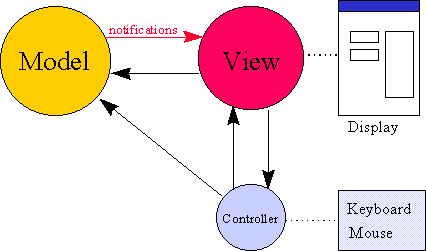
\includegraphics[width=0.9\textwidth]{./content/pictures/mvc-smalltalk.jpg}
	\caption[Classical Model-View-Controller concept as used in Smalltalk.]{Classical Model-View-Controller concept as used in Smalltalk. Model and View know each other.}
	\label{fig:mvc-smalltalk}
\end{figure}

\subsection{Model-View-Presenter}
The Model-View-Presenter (MVP) pattern is similar to the MVC-model as it shares the concept of separating the application into three layers. The responsibilities between the two patterns differ considerably, as can be seen in Figure \ref{fig:mvp}. The view only communicates with the presenter and does not know about the model. The presenter handles user input and requests, gathers data from the model, updates it and finally is responsible for refreshing the view with new data. This implies that the model does not know about the existence of view or presenter and at least in the original concept of MVP all business logic is placed in the presenter classes \cite{mvp}. It is important to note that it is vital for the use of this pattern to implement it using interfaces. This ensures that its main goal, easy testability, can be reached easily. 

\begin{figure}[htbp]
	\centering

	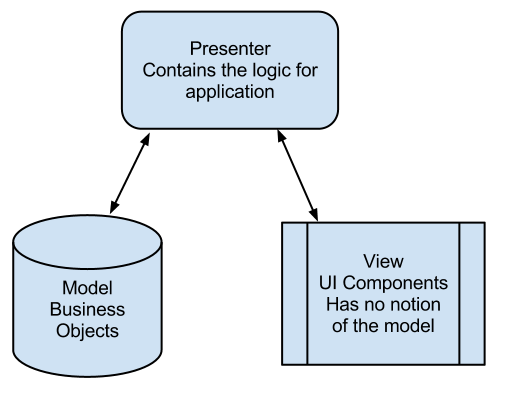
\includegraphics[width=0.7\textwidth]{./content/pictures/mvp.png}
	\caption[Diagram of Model-View-Presenter.]{Diagram of Model-View-Presenter. The view only holds the means for displaying the data and interacting, in opposite to the MVC-model it does not know about the model, but only corresponds with the presenter. The presenter is responsible for gathering the necessary data from the model and forwards it to the view. The model does not know about the presenter.}
	\label{fig:mvp}
	\caption*{Source: \href{https://commons.wikimedia.org/w/index.php?curid=19794348}{https://commons.wikimedia.org/w/index.php?curid=19794348}, accessed on 5.9.2017}
\end{figure}


After some years Martin Fowler drafted two design patterns that are closely connected to MVP. In his blog entry \footnote{\href{https://martinfowler.com/eaaDev/ModelViewPresenter.html}{https://martinfowler.com/eaaDev/ModelViewPresenter.html}} he explained that he felt the need to split the MVP-pattern into two resulting in the following concepts, briefly described in Figure \ref{fig:passive-view-supervision-controller}. 

\begin{figure}[htbp]
	\centering

	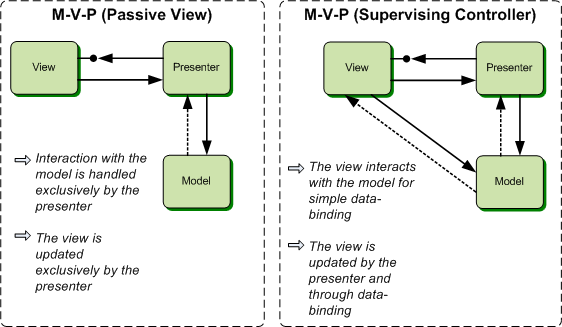
\includegraphics[width=\textwidth]{./content/pictures/passive-view.png}
	\caption[Basic diagrams of the Passive View and Supervising Controller patterns.]{Basic diagrams of the Passive View (left) and Supervising Controller patterns (right). In the former as little logic as possible is placed in the view making it easy replaceable by a mock object for testing. Synchronization logic needs to be placed in the Presenter. In the latter view and model are connected trough data bindings empowering these two to perform synchronization tasks on their own. This simplifies the role of the presenter.}
	\label{fig:passive-view-supervision-controller}
	\caption*{Source: \href{https://msdn.microsoft.com/en-us/library/ff709839.aspx}{https://msdn.microsoft.com/en-us/library/ff709839.aspx}, accessed 5.9.2017}
\end{figure}

\subsubsection{Supervising Controller}
In this concept it is the views responsibility to perform data synchronization using shared classes between it and the model. This simplifies the tasks to be performed by the presentation layer while reducing the level of testability possible. 
\subsubsection{Passive view}
In the concept of passive view the model is not connected with the view, which in terms only corresponds with the presenter. It is desired to minimize the logic placed in the view, leaving it (as the name describes) passive and therefore easy to mock. This is especially useful for automated testing, as it allows the tester not only to test the basic logic placed in the presenter but also its synchronization capabilities. The drawback of this clearly lies in the additional responsibilities that need to be met by the presenter \footnote{\href{http://www.wildcrest.com/Potel/Portfolio/mvp.pdf}{http://www.wildcrest.com/Potel/Portfolio/mvp.pdf}, accessed 4.9.2017}.


\subsection{Client-Server}
The Client-Server model describes a way to separate tasks within a network. While the client, which can be any kind of computer program, requests a resource from the server. It is designated to be used within the internet and is still on of the cornerstones of current web infrastructure \cite[p. 3ff]{server}. A prominent example of the client-server model is the Domain-Name-System (DNS). When a user types in the domain name of a service he wants to access, the browser needs to translate the name into a IP-Address it can work with. In order to do that the browser sends a request to a DNS-Server, making it a client. While it does not need to know how exactly the resolving takes places he requires the server response to have a certain format described in the communication protocol. 

There are several benefits of using this architecture. For example it centralizes the administration which lowers the efforts of managing access rights, accounts and so on. Because the important data is in one place it is easier to create backups and ensure security policies. However a server is considered a \emph{Single Point of Failure}, meaning that a whole service will be unavailable if the server for any reason is not reachable, making it a worthy target of attacks. While the impact depends on the actual service built, scalability and extensibility are important factors. It is easier to extend the features provided by a service when using the client-server-model, while it reduces scalability as the hardware needs to be upgraded from time to time to meet a increased number of requests directed to the server.
\begin{figure}[htbp]
	\centering
	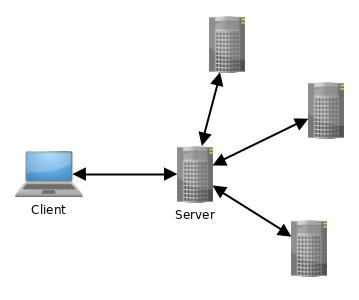
\includegraphics[width=0.7\textwidth]{./content/pictures/client-server.jpg}
	\caption[Client-Server setup.]{Client-Server setup. The client sends a request to a server by messages defined in the protocol. The processing of the request is transparent to the client, it does not know about actions taken by the server and awaits a response in a certain format.}
\end{figure}

\subsection{Peer-to-Peer}
Peer-to-Peer (P2P) infrastructure is the counterpart of client-server-models. No central server exists which means that each of the clients are equally featured, each client has the means to request and provide resources. P2P-Networks are considered more robust and scalable than Client-Server set-ups, as the failure of one node does not lead to the breakdown of the whole system. In picture \ref{fig:p2p} a typical P2P-setup can be seen. 

\begin{figure}[htbp]
	\centering
	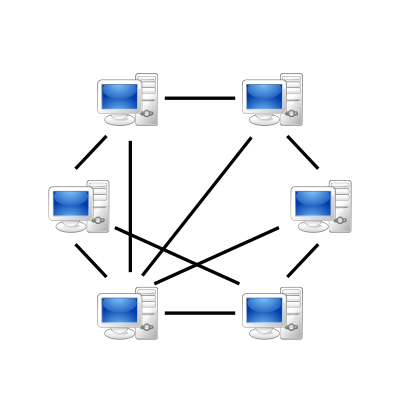
\includegraphics[width=0.7\textwidth]{./content/pictures/P2P-network.jpg}
	\caption[Peer-to-peer setup.]{Peer-to-peer setup. Each peer has the same role, no central server exists.}
	\label{fig:p2p}
	\caption*{Source: \href{https://commons.wikimedia.org/w/index.php?curid=2551723}{https://commons.wikimedia.org/w/index.php?curid=2551723}, accessed on 6.9.2017}
\end{figure}

\subsection{Multi-Tier and Multi-Layer Architecture}
\label{sec:multi-tier}
Multi-Tier architecture is often mentioned in the context of web applications. In general it describes the separation of responsibilities on different \emph{physical} places \footnote{In this context physical separation means that there has to be going on any kind of communication between independent processes within the same machine or connected trough the internet.}. This is the main difference to a multi-layer-system where the responsibilities are separated but placed at the same process which indicates the use of interfaces. 

A 3-Tier-Architecture nowadays refers mostly to the typical set-up of a web application as it can be seen in Figure \ref{fig:multi-tier}. It has to be noted that it is very common to use multi-tier and multi-layer architecture mutually. For example, the logic tier in the figure could use a data-access-layer to abstract the communication with the data tier. 

\begin{figure}[htbp]
	\centering
	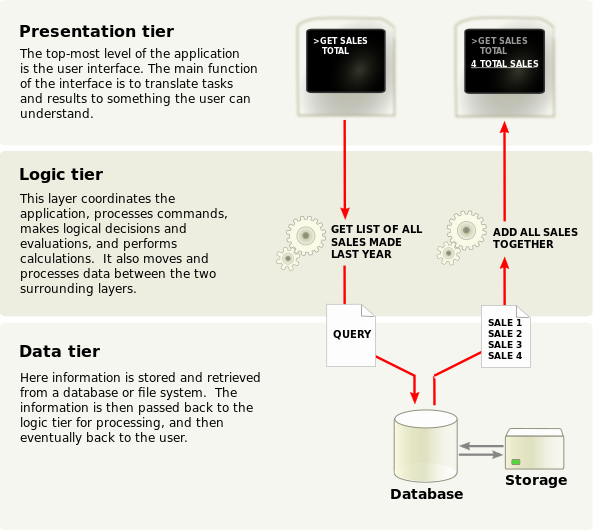
\includegraphics[width=\textwidth]{./content/pictures/multi-tier.jpg}
	\caption[Multi-Tier set-up.]{Multi-Tier set-up. The tiers are physically separated.}
	\label{fig:multi-tier}
	\caption*{Source: \href{https://en.wikipedia.org/wiki/Multitier\_architecture}{https://en.wikipedia.org/wiki/Multitier\_architecture}, accessed on 6.9.2017}
\end{figure}

\section{Technologies}
\subsection{Java}
This project is written in Java, an object oriented programming language released by Sun Microsystems in 1995  \footnote{\href{https://java.com/en/download/faq/whatis_java.xml}{https://java.com/en/download/faq/whatis\_java.xml}, accessed 7.9.2017}. In 2010 the company Oracle bought it and is developing and distributing the language since. It is split up into two main components, its development kit (JDK) and its runtime environment (JRE). The JRE is providing a virtual environment called Java Virtual Machine (JVM) which is used to run so-called Java Bytecode which is comparable to x86 assembler. This bytecode can be compiled from plain Java programs as well as other languages such as Scala or Groovy. 
This approach helps reaching one major goal of the language: portability. Java bytecode can be executed on every platform, as long as a JRE is installed, which nowadays includes mobile phones, embedded platforms and with reduced functionality even smart cards \footnote{\href{http://www.oracle.com/technetwork/java/embedded/javacard/overview/index.html}{http://www.oracle.com/technetwork/java/embedded/javacard/overview/index.html}, accessed 7.9.2017}. 

The JRE uses an interpreter and a just-in-time (JIT) compiler to generate native machine code that can be executed of the platforms processor. A JIT-Compiler generates the necessary machine code at runtime for some parts of the application. This can lead to significant performance improvements compared to the exclusive use of an interpreter.

As of September 2017 according to the TIOBE-Index it is the most popular programming language with a share of more than 12\% \footnote{\href{https://www.tiobe.com/tiobe-index/}{https://www.tiobe.com/tiobe-index/}, accessed 7.9.2017}. 
\subsection{Swing}
\label{sec:swing}
Swing is a Graphical-User-Interface (GUI) Library for Java and was first published in 1997. It is rendered directly by Java thus it is not necessary for a platform to provide specific controls. However this leads to a significant difference in appearance to applications natively written for the platform as some control concepts may differ or buttons may be placed at other positions. This problem is bypassed by the introduction of different \emph{Look-and-Feels} which intend to adopt the application to be as similar to a native program as possible.

\subsection{JavaFX}
\label{sec:javafx}
JavaFX is a framework \footnote{The main difference between a framework and a library is the so-called \emph{Inversion of Control}. While a library is called by the programmer, when using a framework it is in control and calls methods provided by the developer.} for GUI programming in Java and was released in 2014, replacing Swing as the main method for graphical programming. In opposite to Swing it implements its own multimedia-stack able to access graphics card feature through OpenGL and Windows Direct3D.  

\subsection{Relational Databases and PostgreSQL}
\label{sec:postgres}
PostgreSQL is a open source object-relational database management system (ORDBMS) that was first published in 2002. Other than many database management systems it is focused on maintaining a good SQL standard compliance and is currently ranked as the 4th most popular engine. \footnote{ \href{https://www.postgresql.org/about/}{https://www.postgresql.org/about/}, accessed 7.9.2017} \footnote{\href{https://db-engines.com/de/ranking}{https://db-engines.com/de/ranking}, accessed 7.9.2017}

Almost all database systems that are considered as relational use the Structured Query Language (SQL) or a dialect of it as language for querying and manipulating the database. Such a system is characterized by structuring the data into \emph{tables}, which consists of \emph{columns} and \emph{rows} (also: \emph{records}). Many systems require each row to have a unique identifier, also called \emph{primary key}. This key can consist of one or more columns per row, if more columns are considered it is also called \emph{composite key}. 

If it is wanted to refer from one table row to the a record from another table a \emph{foreign key} is used which corresponds to the primary key of the original table. This is vital for maintaining the so-called \emph{referential integrity}, which indicates that all references have valid targets. Depending on the policy set in the database management system or specified in the foreign key definition of the table the deletion of a row that is referred by another record could be prevented.


\subsection{MongoDB}
\label{sec:mongodb}
As a prominent example for NoSQL\footnote{Not only SQL}-databases MongoDB is a database engine written in C++ and published in 2009. In opposite to relational databases it persists the data in \emph{documents} which are structured in a JSON\footnote{JavaScript Object Notation, a syntax for exchanging data which is easy to read for humans and efficiently processable by machines. It is build around key-value-pairs which can be nested.}-like manner. 

Documents can be stored in \emph{collections}, which are comparable to tables in SQL-databases. While all rows in tables possess the same columns this is not necessarily true for collections. Each document in a collection can hold arbitrary attributes which improves the flexibility while as a trade-off reducing data integrity. In opposite to relational databases in MongoDB foreign keys cannot be created, however each document is provided with a built-in unique identifier.

\subsection{Caching}

Caching is the process to hold often needed data in memory to reduce the time necessary for gathering. While most of modern database management systems already provide advanced caching techniques out of the box, the application could be physically separated from the server by a low-bandwidth network. Therefore client-side caching may be necessary for reducing latency. 

In most of the cases placing the cache in the data access layer (see section \ref{sec:multi-tier}) leads to the simplest implementation as all data accesses are passing through here, however depending on the structure and needs of the application it may be necessary to implement the cache in the business code.

\subsubsection{Caching strategies}
There are two main types of caching policies: \emph{write-through} and \emph{write-back}. When performing write-trough-caching all data is first persisted and then immediately updated in the cache while blocking the operation until all necessary writes are completed. This ensures that at all times a up-to-date copy of the data is available \footnote{\href{http://searchsolidstatestorage.techtarget.com/answer/Comparing-write-through-write-back-and-write-around-caching}{http://searchsolidstatestorage.techtarget.com/answer/Comparing-write-through-write-back-and-write-around-caching}, accessed 10.9.2017}. 

The write-back-policy on the other hand also caches write accesses without directly persisting it. The write operation onto the data tier is being performed asynchronously, this may then happen when the system load is low and therefore the overall performance may be improved. However it is considered more dangerous in terms of data loss due to system crashes or other errors as the only valid copy of the data is only resided in the cache  \footnote{\href{http://www.computerweekly.com/feature/Write-through-write-around-write-back-Cache-explained}{http://www.computerweekly.com/feature/Write-through-write-around-write-back-Cache-explained}, accessed 10.9.2017}.

\subsubsection{Cache Replacement Policies}
As memory is a scare resource it is necessary to limit caching space and thus not all data can be cached at the same time. This introduces the necessary of means to decide which cache entries are to abolish, this mechanism is called a \emph{Cache Replacement Policy}. 

The best policy clearly would be to replace the cache entry that will be needed again the latest. As this is information that is not available the associated \textbf{Bélády's algorithm} is considered theoretical and is only used for measuring and comparing the performance of other policies.

There are several possibilities which differ significantly depending on the data access pattern (this list is not exhaustive):
\begin{itemize}
	\item \textbf{First-In, First-Out (FIFO)}: When caching with the FIFO policy as soon the cache runs full the \emph{oldest} entry will be replaced. This is typically implemented as a Queue because it reduces the efforts to keep track of the entries age.
	\item \textbf{Least Recently Used (LRU)}: This algorithm keeps track of the last reference to cache entries. When a replacement is necessary it frees the page which reference dates back the longest. 
	\item \textbf{Least Frequently Used (LFU)}: Research has shown that LRU performs poorly for some access patterns, so instead of deciding which page is to replace upon the access time, LFU decides upon the number of accesses.
	\item \textbf{Most Recently Used (MRU)}: Access patterns exist where it is preferred to abolish the entry that was accessed most recently, an example for this scenario would be the sequentially scanning of a file. The implementation is very similar to LRU.
	\item \textbf{Random}: Interestingly research has shown that random replacement can be considered a good strategy as well, especially as it is easy to implement and efficient. Most of the more advanced policies may perform better with certain access patterns while performing worse in others. In many cases it is not possible to predict how the accesses will take place which introduces the risk of experiencing a unfavourable pattern. Random replacement is not sensitive to this problems while providing solid performance.
\end{itemize}

\subsubsection{Cache invalidation}
In the context of cache invalidation a quote which is said to come from Phil Karlton is especially famous:
\begin{quote}
There are only two hard things in Computer Science: cache invalidation and naming things.
\end{quote}

A Cache invalidation mechanism is necessary if the data tier can be updated from more than one location or clients which is especially in the terms of web application the standard case. 

Most caching strategies therefore feature a so-called time based expiry. It provides each cache record with a time-out after that it will be evicted \footnote{\href{http://tutorials.jenkov.com/software-architecture/caching-techniques.html}{http://tutorials.jenkov.com/software-architecture/caching-techniques.html}, accessed 10.9.2017}

Another method is active cache invalidation which evicts either cache entry or the whole cache after a change in the data tier. To support this some kind of messaging mechanism is necessary to let the persistent storage notify all clients about the update. 

In the case of multiple clients it has to be noted that it could be desirable to store additional version information for the table rows, for instance a incrementing counter or a hash of the data set. Because of the possibility of multiple clients updating the same row concurrently from different locations race conditions can occur that lead to the overwriting of newly entered data. Even with active cache invalidation it cannot be guaranteed that the update notification reaches the second client in-time. 
\chapter{Methods}

\section{Domain Description}
As stated before the application should provide a time-tracking solution for commercial projects.
Therefore it is divided into three general areas:
\begin{itemize}
\item \textbf{Project}: A project is the overall term for a distinguishable amount of work that is done for a specific customer.
\item \textbf{Phase}: Each project exists of one or more phases that are used to monitor the progress of the project.
\item \textbf{Activity}: A activity represents a workload that is done by a specific member in a specific phase for a specific project.
\end{itemize}
In this application, two basic roles exist.
\begin{itemize}
\item \textbf{Project Leader}: A project leader has the responsibility of maintaining project specific data, such as description, phases and assigning project members. He is \emph{not} allowed to create new users. After creating a new project, one is automatically project leader. A project leader is allowed to monitor the statistics of his projects including the workloads of the project members
\item \textbf{Member}: As a simple member one is allowed to add, delete and modify activities created by the user. A member is only allowed to perform this actions for projects he is assigned to. He is also only allowed to monitor his own statistics.
\end{itemize}

\subsection{Use-Cases}
\subsubsection{General Use-Cases}
\begin{enumerate}
\item \textbf{Login:} After starting the program, a login prompt shall show up. The user provides his credentials which will be compared to the saved credentials in the database. If they are correct, he is forwarded to the main program.\\
The user has the possibility to reset his password by activating a button and providing his email-address. A new password will be sent to the address, if a user with this address is known by the system. 

\item \textbf{Starting / Stopping activities:} Through a banner at the top of the program each user can select a project he is assigned to and furthermore a phase of this project. After providing a name of the activity he can start the activity by clicking on a start button. The same button can be used to stop the activity. After stopping (or closing the application), the activity is complete and is added to the database and project statistics.

\item \textbf{Personal statistics:} Utilizing the associated button of the left side bar the main panel lists all project the user is assigned to and the time he spent working for these projects. At the top of the main panel he can choose the period he wants to see. After clicking on one of the entries a statistic of the working time for each phase of the project is shown. By clicking at a phase all activities in this phase are listed and can be modified and deleted, furthermore a new activity can be created here too. By clicking on a button at the top the user can switch the view to the previous view.

\item \textbf{Create and manage projects:} Each user can create new projects by using the associated button of the left side bar. The main panel then lists all projects which project leader he is. After clicking on a entry, the main window shows the details of the project, such as the description, the created phases and the project members. He is able to perform all necessary operations associated with the project in this view, as well as declaring a new project leader.

\item \textbf{Settings:} Utilizing the associated button of the left side bar the main panel provides means to change the password, email-address and name.
\end{enumerate}
\subsubsection{Project leader Use-Cases}
\begin{enumerate}
\item \textbf{Project statistics:} Other than normal users, a project leader can monitor the statistics of all of his projects by using the according button on the side bar. The main panel lists all projects he is leader of. After choosing one project he can choose the period he is interested in at the top of the panel. At the left side of the main window now all project members are listed. After choosing one or more project members, the time they spent working for the different phases of the project is listed at the center.
\end{enumerate}


The persistent storage has a quite simple structure, as can be seen in figure \ref{fig:database}. It is notable that the roles are described as text and therefore are human-readable. 
\begin{figure}[htbp]
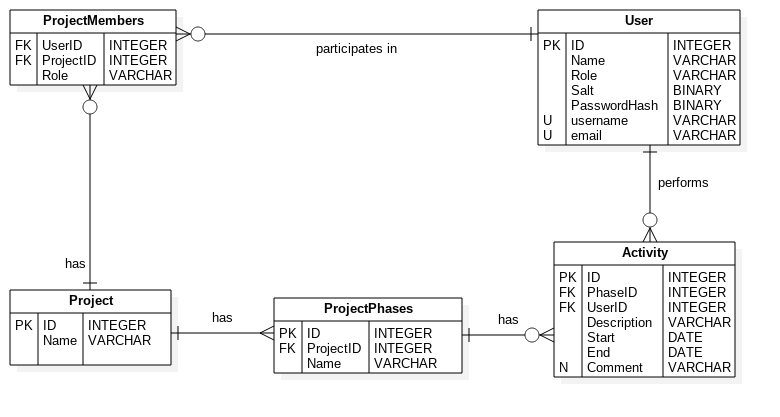
\includegraphics[width=\textwidth]{./content/pictures/database.png}
\caption{Database diagram}
\label{fig:database}
\end{figure}

\clearpage

\section{Phase 1: One Databse and UI}
\subsection{Monolithic Code Samples}
%\subsubsection{Database Access}
%\subsubsection{UI Interaction}

\subsection{Best-Practice Code Samples}
%\subsubsection{Database Access}
%\subsubsection{UI Interaction}

\section{Phase 2: More Databases / UIs}

\subsection{Monolithic Code Samples}
%\subsubsection{Database Access}
%\subsubsection{UI Interaction}

\subsection{Best-Practice Code Samples}
%\subsubsection{Database Access}
%\subsubsection{UI Interaction}
\chapter{Results}
\label{sec:results}
In order to make serious statements about the quality of the code and the effects of using the design patterns some indicators were chosen to compare the two application types. Because the two programs are similar in its work-flow and basic structure these comparisons are actually meaningful.

This section only lists the findings while section \ref{sec:discussion} puts the results into context and explains them.

\section{Lines of Code}
\label{sec:line-count}
In Table \ref{table:lines-of-code} the total lines programmed for both programs and the phases are listed. This is counted by using simple command-line on the different branches of the program. In figure \ref{fig:lines-of-code} the  increase in lines of code can be seen. It is notable that the best practice implementation consists of more total lines of code in all phases. 

Due to the use of interfaces in java a lot of annotations were necessary which in fact do not have any significance to the topic. Thus the adjusted line count excludes lines that only hold the \texttt{@Override}-Annotation.

\begin{table}[htbp]
	\centering

	\begin{tabular}{|c|c|c|c|c|} \hline
	\textbf{Program version} &\textbf{Phase 1} & \textbf{Phase 2} & \textbf{Phase 3} \\ \hline
	Best practice & 9264 & 12275 (+ 32\%)& 13306 (+ 8\%)\\ \hline
	Best practice (adjusted) & 8804 & 11764 (+ 34\%)& 12750 (+ 8\%)\\ \hline
	Ad-hoc & 7572 & 11172 (+ 48\%)& 12168 (+ 9\%)\\ \hline
	\end{tabular}
	\caption{Lines of code for both program versions and all phases}
	\label{table:lines-of-code}
\end{table}

\begin{figure}[htbp]
	\centering

	\begin{tikzpicture}
	\begin{axis}[
	height=0.7\textwidth,
	xlabel={Phases},
	ylabel={Lines of Code},
	y label style={at={(axis description cs:-0.1,.5)}},
	xmin=0, xmax=4,
	ymin=6000, ymax=14000,
	xtick={1,2,3},
	ytick={6000, 8000, 10000, 12000, 14000},
	legend pos=south east,
	ymajorgrids=true,
	grid style=dashed,
	scaled ticks=false, 
	tick label style={/pgf/number format/fixed} 
	]
	
	\addplot[
	color=blue,
	mark=x,
	]
	coordinates {
		(1,9205.0)(2,12275.0)(3,13306.0)
	};
	
	\addplot[
	color=green,
	mark=*,
	]
	coordinates {
		(1,8804)(2,11764)(3,12750)
	};

	\addplot[
	color=red,
	mark=square,
	]
	coordinates {
		(1,7572)(2,11172)(3,12168)
	};
	\legend{Best Practice, Best Practice (adjusted), Ad-hoc}
	
	\end{axis}
	
	\end{tikzpicture}
	\caption[Lines of Code for both program versions and all phases.]{Lines of Code for both program versions and all phases. The best practice implementation of the program both in the adjusted and original version consists of more code lines in all phases.}
	\label{fig:lines-of-code}
\end{figure}


\section{Touched and Edited Files}
\label{sec:file-count}
The development of the file count is listed in this section. Table \ref{table:files} and figure \ref{fig:files} shows how many files are needed for the programs while table \ref{table:touched-files} list the number of files that were modified or created during the implementation of the requirements.

\begin{table}
	\centering
	\begin{tabular}{|c|c|c|c|c|} \hline
		\textbf{Program version} &\textbf{Phase 1} & \textbf{Phase 2} & \textbf{Phase 3} \\ \hline
		Best practice & 96 & 125 & 131 \\ \hline
		Ad-hoc & 59 & 88 & 89 \\ \hline
	\end{tabular}
	\caption{Total number of files for both program versions and all phases}
	\label{table:files}
\end{table}

\begin{figure}
	\centering

	\begin{tikzpicture}
	\begin{axis}[
	xlabel={Phases},
	ylabel={Total number of files},
	y label style={at={(axis description cs:-0.1,.5)}},
	xmin=0, xmax=4,
	ymin=50, ymax=150,
	xtick={1,2,3},
	ytick={50, 70, 90, 110, 130, 150},
	legend pos=south east,
	ymajorgrids=true,
	grid style=dashed,
	scaled ticks=false, 
	tick label style={/pgf/number format/fixed} 
	]
	
	\addplot[
	color=blue,
	mark=square,
	]
	coordinates {
		(1,96)(2,125)(3,131)
	};
	
	\addplot[
	color=red,
	mark=square,
	]
	coordinates {
		(1,59)(2,88)(3,89)
	};
	\legend{Best Practice, Ad-hoc}
	
	\end{axis}
	
	\end{tikzpicture}
	\caption{Total number of files for both program versions and all phases}
	\label{fig:files}
\end{figure}

 \begin{table}
 	\centering

 	\begin{tabular}{|c|c|c|} \hline
 		\textbf{Program version} &\textbf{Phase 1 to Phase 2} & \textbf{Phase 2 to Phase 3} \\ \hline
 		Best practice & 30 & 7 \\ \hline
 		Ad-hoc & 39 & 13\\ \hline
 	\end{tabular}
 	\caption{Number of files modified or added for both program versions and all phases} 	\label{table:touched-files}
 \end{table}

\section{Average line count per file}
\label{sec:avg-line-count}
Another interesting aspect of the data is the comparison of the average line count per file, as it can be seen in table \ref{table:avg-lines} and chart \ref{fig:avg-lines}. The results are rounded.

\begin{table}
	\centering

	\begin{tabular}{|c|c|c|c|} \hline
		\textbf{Program version} &\textbf{Phase 1} & \textbf{Phase 2} & \textbf{Phase 3} \\ \hline
		Best practice & 96 & 98 & 102 \\ \hline
		Best practice (adjusted) & 92 & 94 & 97\\ \hline
		Ad-hoc & 128 & 127 & 137 \\ \hline
	\end{tabular}
	\caption{Average lines per file for both program versions and all phases}
	\label{table:avg-lines}
\end{table}

\begin{figure}

	\centering
	\begin{tikzpicture}
	\begin{axis}[
	xlabel={Phases},
	ylabel={Lines of Code per file},
	y label style={at={(axis description cs:-0.1,.5)}},
	xmin=0, xmax=4,
	ymin=50, ymax=150,
	xtick={1,2,3},
	ytick={50, 70, 90, 110, 130, 150},
	legend pos=south east,
	ymajorgrids=true,
	grid style=dashed,
	scaled ticks=false, 
	tick label style={/pgf/number format/fixed} 
	]
	
	\addplot[
	color=blue,
	mark=square,
	]
	coordinates {
		(1,96)(2,98)(3,102)
	};

	\addplot[
	color=green,
	mark=square,
	]
	coordinates {
		(1,92)(2,94)(3,97)
	};
	
	\addplot[
	color=red,
	mark=square,
	]
	coordinates {
		(1,128)(2,127)(3,137)
	};
	\legend{Best Practice, Best Practice (adjusted), Ad-hoc}
	
	\end{axis}
	
	\end{tikzpicture}
	\caption{Average lines of code per file for both program versions and all phases}
	\label{fig:avg-lines}
\end{figure}

\chapter{Discussion}
\label{sec:discussion}
In this chapter all data gathered in the last section is revisited and put into context. 
\section{Meaning and significance of the file count}
As clearly visible in section \ref{sec:file-count} the ad-hoc version of the program does not need as many files as the best practice implementation. This is mainly due to the missing interface files, as well as the files for repositories. Especially in phase 3, where a new database should be supported, this factor can be easily observed. In the ad-hoc version all code concerning the database interaction was put into existing classes, resulting in only one additional file while the best practice implementation needs to create and derive one file per repository. 

\section{Meaning and significance of the line count}
The same statement as above applies to the count of total lines as seen in section \ref{sec:line-count}. Each interface class consists of various method declarations that are counted as well. As stated in section \ref{sec:line-count} for better comparison in addition to the total line count for the best practice implementation another count was made excluding the \texttt{@Override}-Annotation lines as they bias the result. 

Here a interesting observation can be made for the line count: While the total count of the best practice version is higher for both phases 1 and two, the increase of lines is between the phases is significantly lower. While the best practice version added 2960 lines of code, the ad-hoc version added 3600 lines of code. This difference of about 700 lines does not seem much, however it has to be noted that this lines were mainly necessary because of case distinctions as can be seen in section \ref{sec:ad-hoc-javafx}. This reduces readability on the one hand and results in a greater risk of programming errors. 

The fact that the increase in lines between phase 2 and 3 is nearly the same is easily explained as the added files differ significantly. This is due to the overhead of declaring a class including its constructor and other programming-language-connected actions which lead to a high number of additions which are not necessary in the ad-hoc version.

Additionally to the lower number of files and the comparable number of lines in the two programs, the ad-hoc implementation on average contains noticeably more code per file. As the two implementations offer exactly the same functionality this means that responsibilities have shifted and each class is in charge of more actions. However this fact is a clear violation of the Single-Responsibility-Principle (see section \ref{sec:srp}) which may introduce more programming errors in the future. 

\section{Maintainability}
The biggest effect and difference when using design patterns and interfaces can be observed exactly in conforming of the Single-Responsibility-Principle and hence in the readability of the code. While each data class of the ad-hoc version does not only have the responsibility to encapsulate the data, it is responsible for saving the data to two different kinds of persistent storage. This results in a quite long file that mixes technologies and needs to be revisited any time a new persistent storage is added, existing storage technologies are changed or the data classes change. 

In the case of view frameworks due to missing use of interfaces asides from implementing the view using a new framework each and every class that depends on any kind of interface needs to be adopted. This is visible in table \ref{table:touched-files}, where is stated that the implementation of new technologies influences lower numbers of dependent files which is a very desired behaviour. 

In addition to the points mentioned above the metric of the code complexity which can be seen in section \ref{sec:complexity} clearly indicates a difference in the maintainability of the application. The cyclometric complexity states the independent paths in a program, a higher number indicates that the code is on the one hand difficult to understand and on the other hand is more likely to contain errors\footnote{\href{http://www.chambers.com.au/glossary/mc\_cabe\_cyclomatic\_complexity.php}{http://www.chambers.com.au/glossary/mc\_cabe\_cyclomatic\_complexity.php}}. Furthermore as some testing strategies are targeting to cover all paths of a program a higher code complexity may also lead to higher testing effort.

Similar to the results of the straight-forward line count the complexity development seen in table \ref{table:total-complexity} shows that while the initial complexity of the ad-hoc program version is slightly lower especially in the transition from phase 1 to phase 2 the complexity raises over-proportionally compared to the best-practice implementation. 
Also the code complexity per file as can be seen in table \ref{table:file-complexity} shows that due to the reduced number of files each file has a quite high complexity. This indicates that the classes are more difficult to understand and test which impacts maintainability negatively. 
\chapter{Conclusion}

In the last chapters some interesting findings were gathered. Two program versions were compared, one following best practice guidelines in the sense of object oriented programming, the other one featured ad-hoc programming without paying attention to topics of software maintenance.

Throughout the development process five major issues could be discovered:

\begin{itemize}
	\item \textbf{Number of files}: The best practice version of the application needed a higher number of files than the ad-hoc implementation throughout all phases.
	\item \textbf{Lines of code}: The best practice version needed more lines of code in all phases.
	\item \textbf{Lines per file}: The best practice versions files contained notably less lines of code per file.
	\item \textbf{Increase in code lines}: Especially in transition from phase 1 to phase 2 the best practice implementation needed considerably less code additions.
	\item \textbf{Touched files}: The number of touched or edited files during phase traversal was lower in the best practice program version.
\end{itemize}

It has to be said that the results gathered in section \ref{sec:results} may vary depending on the coding style, programming language, concrete use case and size of the project, furthermore the term \emph{code quality} does not have a unique definition. There are many different standpoints on what attributes a well written code should have, often depending on company coding policies. One factor that is not mentioned by intention in this thesis is the readability of the code as this is a very subjective matter and is therefore not considered. 

In terms of the definition used in this thesis, which mainly focuses on properties defined by guidelines of the object oriented programming the results support the hypothesis saying that the use of design patterns improves code quality in later stages of a project cycle. This is backed up by the lower number of files needing modification in the process of extending functionality and the lower number of lines added between phases 1 and 2 as well as the increase in code complexity between those two phases.

At the same time in the first stage the initial programming effort for a clean implementation using well-known patterns is considerably higher, and even later on in the best practice implementation utilizes both a larger number of files and more lines of code, which may increase the efforts for software maintenance and testing.

In conclusion it can be said that the use of design patterns can help to increase code quality if the requirements of a software project are likely to change, which is the common case especially for bigger applications. 

As this work only focuses on a small number of design patterns and other literature does not come to clear results as well, further research is certainly necessary. If future work is focusing on existing software projects, challenges will likely include the difficulties in comparing different approaches applied in the compared applications. However if new research rather studies effects of design patterns by observing controlled experiments, as this thesis does, the main challenge will likely include the question if small scale results also apply for enterprise scale applications.


%\chapter{Future Work}
\section{Physical Seperation of Tiers}

\cleardoublepage

\appendix
\chapter{Source Code}
All source code including this thesis is online available on Github \footnote{\href{https://github.com/Vallant/design-patterns-study.git}{https://github.com/Vallant/design-patterns-study.git}} under the GPLv3 licence. \footnote{\href{https://www.gnu.org/licenses/gpl-3.0.de.html}{https://www.gnu.org/licenses/gpl-3.0.de.html}}.

The repository consists of a main branch, a thesis branch and 6 branches corresponding to the phases for each program implementation. The main branch contains the latest version of both applications as well as the latest version of the thesis branch. In the thesis branch naturally only tex sources for creating the thesis can be found. The branches corresponding to the phases are called \texttt{bpV\{1|2|3\}} (best-practice phase 1,2 or 3) and \texttt{monoV\{1|2|3\}} (monolithic phase 1,2 or 3 \footnote{The term monolithic was used in a early stage of development and was later dropped in favour of \emph{ad-hoc}})

In order to run the application, some pre-requirements have to be met. Firstly a PostgreSQL and a MongoDB database must be installed. Secondly the database initialization code that can be found in the directory \texttt{<repository-root>/src/db} needs to be imported into the corresponding DBMS. This code creates the necessary tables, columns, constraints etc. On more information about how to import and the code please refer to the documentation of the two DBMS.

For compiling the application ant build scripts are available, the application jar can be compiled using the following command:

\texttt{ant -f src/<program version>/build.xml}.


To start the program it can be called using the command line utilizing the following command:

\texttt{java -jar <application-name> <driver> <url:port> <username> <password> <controller> <frontend>}

If the current working directory is the repository root, this means that the following commands are available, depending on the branch.

\begin{footnotesize}
	\texttt{java -jar src/monolithic/out/artifacts/monolithic\_jar/monolithic.jar mongo localhost postgres postgres standard javafx}
	
	\texttt{java -jar src/monolithic/out/artifacts/monolithic\_jar/monolithic.jar mongo localhost postgres postgres standard swing}
	
	\texttt{java -jar src/monolithic/out/artifacts/monolithic\_jar/monolithic.jar \\ org.postgresql.Driver jdbc:postgresql://localhost/casestudy  postgres postgres standard javafx} 
	
	\texttt{java -jar src/monolithic/out/artifacts/monolithic\_jar/monolithic.jar\\
		org.postgresql.Driver jdbc:postgresql://localhost/casestudy  postgres postgres standard swing} 
	
	\texttt{java -jar src/best-practice/out/artifacts/best\_practice\_jar/best-practice.jar org.postgresql.Driver jdbc:postgresql://localhost/casestudy  postgres postgres standard javafx
	}

	\texttt{java -jar src/best-practice/out/artifacts/best\_practice\_jar/best-practice.jar mongo localhost  postgres postgres standard javafx
	} 

	\texttt{java -jar src/best-practice/out/artifacts/best\_practice\_jar/best-practice.jar org.postgresql.Driver jdbc:postgresql://localhost/casestudy  postgres postgres standard swing
	} 

	\texttt{java -jar src/best-practice/out/artifacts/best\_practice\_jar/best-practice.jar mongo localhost postgres postgres standard javafx
	} 
\end{footnotesize}





\let\LaTeXStandardClearpage\clearpage
\let\clearpage\relax  % Do nothing when a \clearpage command appears 
\let\cleardoublepage\relax
\printbibliography	
\listoffigures
\listoftables
\lstlistoflistings

\let\clearpage\LaTeXStandardClearpage % Return to the old definition

\end{document}

